\subsection{Eigenspace Overlap Between Different Models}
\label{sec:appendix_expres_ovlp}
The non trivial overlap between top eigenspaces of layer-wise Hessians is one of our interesting observations that had been discusses in \sectionref{sec:models}. Here we provide more related empirical results. Some will further verify our claim in \sectionref{sec:models} and some will appear to be challenge that. Both results will be explained discussed more extensively in \sectionref{sec:appendix_explanation}.

\subsubsection{Overlap preserved when varying hyper-parameters:}
We first verify that the overlap also exists for a set of models trained with the different hyper-parameters. Using the LeNet5 (defined in \tableref{tab:appendix_lenet_struct}) as the network structure. We train 6 models using the default training scheme (SGD, lr=0.01, momentum=0), 5 models using a smaller learning rate (SGD, lr=0.001, momentum=0), and 5 models using a combination of optimization tricks (SGD, lr=0.01, momentum=0.9, weight decay=0.0005).
With these 16 models, we compute the pairwise eigenspace overlap of their layer-wise Hessians (120 pairs in total) and plot their average in \figureref{fig:app_overlap_different_hyperparam}. The shade areas in the figure represents the standard deviation. The pattern of overlap is clearly preserved, and the position of the peak roughly agrees with the output dimension $m$, demonstrating that the phenomenon is caused by a common structure instead of similarities in training process.

\begin{figure}[H]
    \centering
    % \vspace{-1em}
    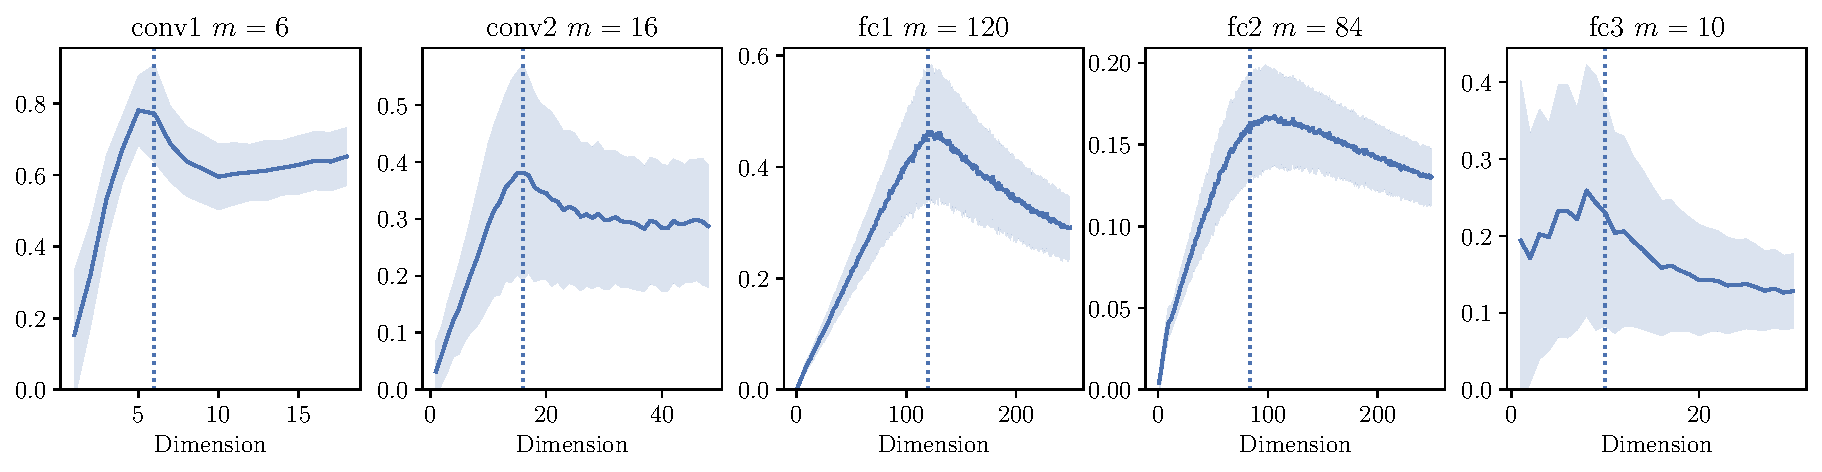
\includegraphics[width=\textwidth]{Appendix_Figures/Overlap_different_models/DimOverlap_CIFAR10_LeNet5_normnew_fixlr0.001_X_LeNet5_normnew_fixlr0.01_X_LeNet5_normnew_fixlr0.01_momentum_appendix_full.pdf}
    \vspace{-1em}
    \caption{Eigenspace overlap of different models of LeNet5 trained with different hyperparameters.}
    \vspace{-1em}
    \label{fig:app_overlap_different_hyperparam}
\end{figure}

Note that for fc3 (the final output layer), we are not observing a linear growth starting from 0 like other layers. This can be explained by the lack of neuron permutation. Related details will be discussed along with the reason for the linear growth pattern for other layers in \sectionref{sec:appendix_model_overlap}.

\subsubsection{Eigenspace overlap for convolutional layers in large models:}
Even though the exact Kroneckor Factorization for layer-wise Hessians is only well-defined for fully connected layers, we also observe similar nontrivial eigenspace overlap for convolutional layers in larger and deeper networks including variants of VGG11 and ResNet18 on datasets CIFAR10 and CIFAR100. Some representative results are shown in \figureref{fig:app_adexp_vgg} and \figureref{fig:app_adexp_resnet}. For each model on each dataset, we independently train 5 models and compute the average pairwise eigenspace overlap. The shade areas represents the standard deviation.
 
For most of the convolutional layers, the eigenspace overlap peaks around the dimension which is equal to the number of output channels of that layer, which is similar to the layers in LeNet5 as in \figureref{fig:app_overlap_different_hyperparam}. The eigenspace overlap of the final fully connected-layer also behaves similar to fc3:LeNet5, which remains around a constant then drops after exceeding the dimension of final output.
However, there are also layers whose overlap does not peak around the output dimensions, (e.g. conv2 of \figureref{fig:app_adexp_vgg}(a) and conv7 of \figureref{fig:app_adexp_resnet}(a)). We will discuss these special cases in the following paragraph.

% \begin{figure}[H]
%     \centering
%     \subfigure[\centering\small{VGG11-W32 (CIFAR10)}]{
%     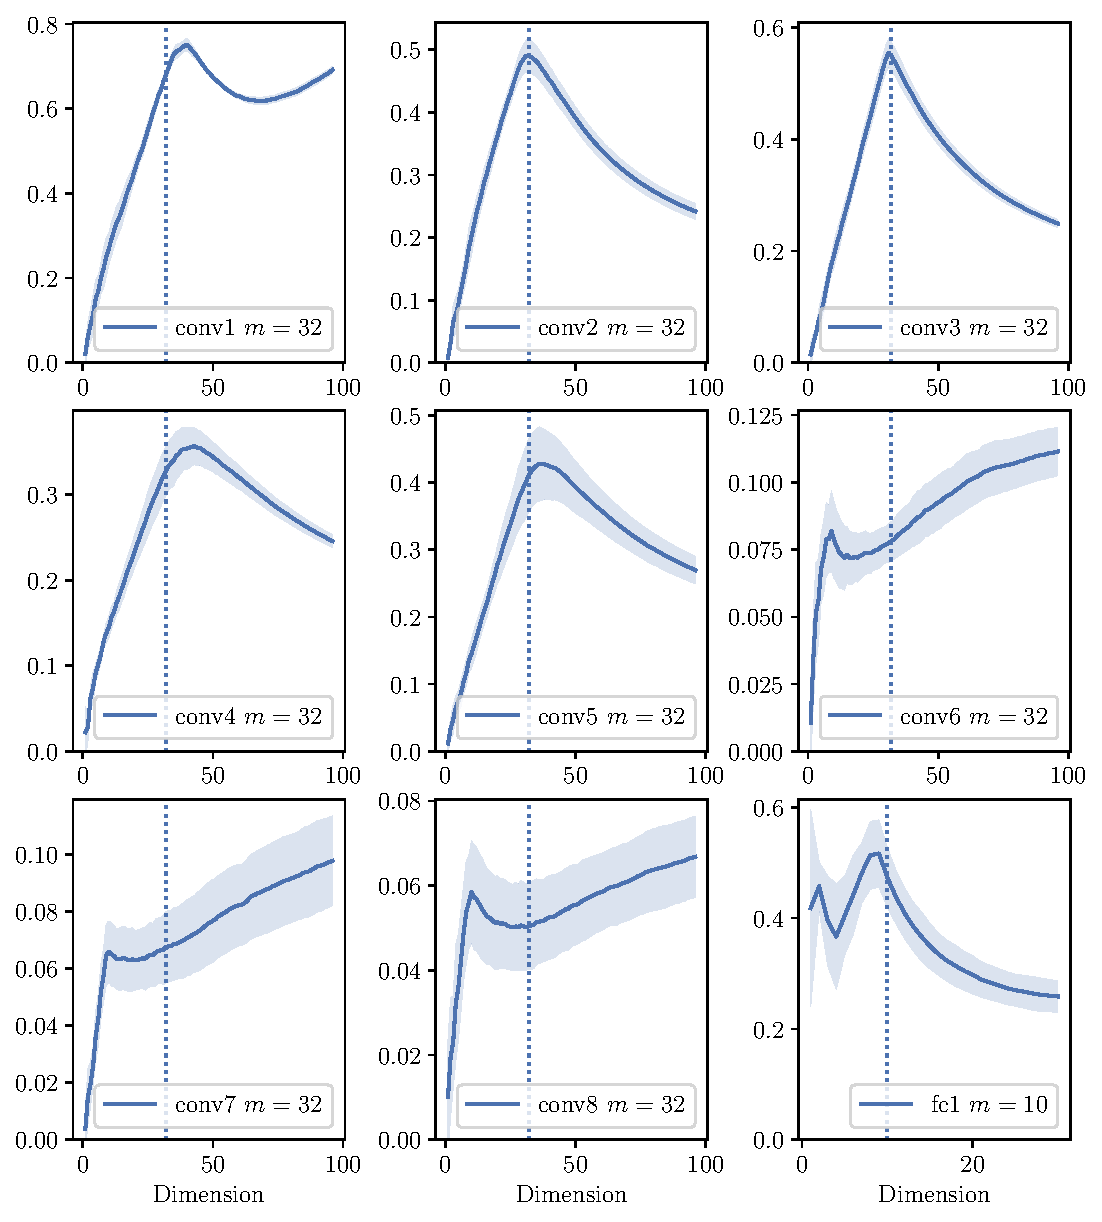
\includegraphics[width=0.48\textwidth]{Appendix_Figures/Overlap_large_model/overlap_raw/DimOverlap_CIFAR10_VGG11W32_fixlr0.01_appendix_vertical_3col.pdf}}
%     \subfigure[\centering\small{VGG11-W200 (CIFAR10)}]{
%     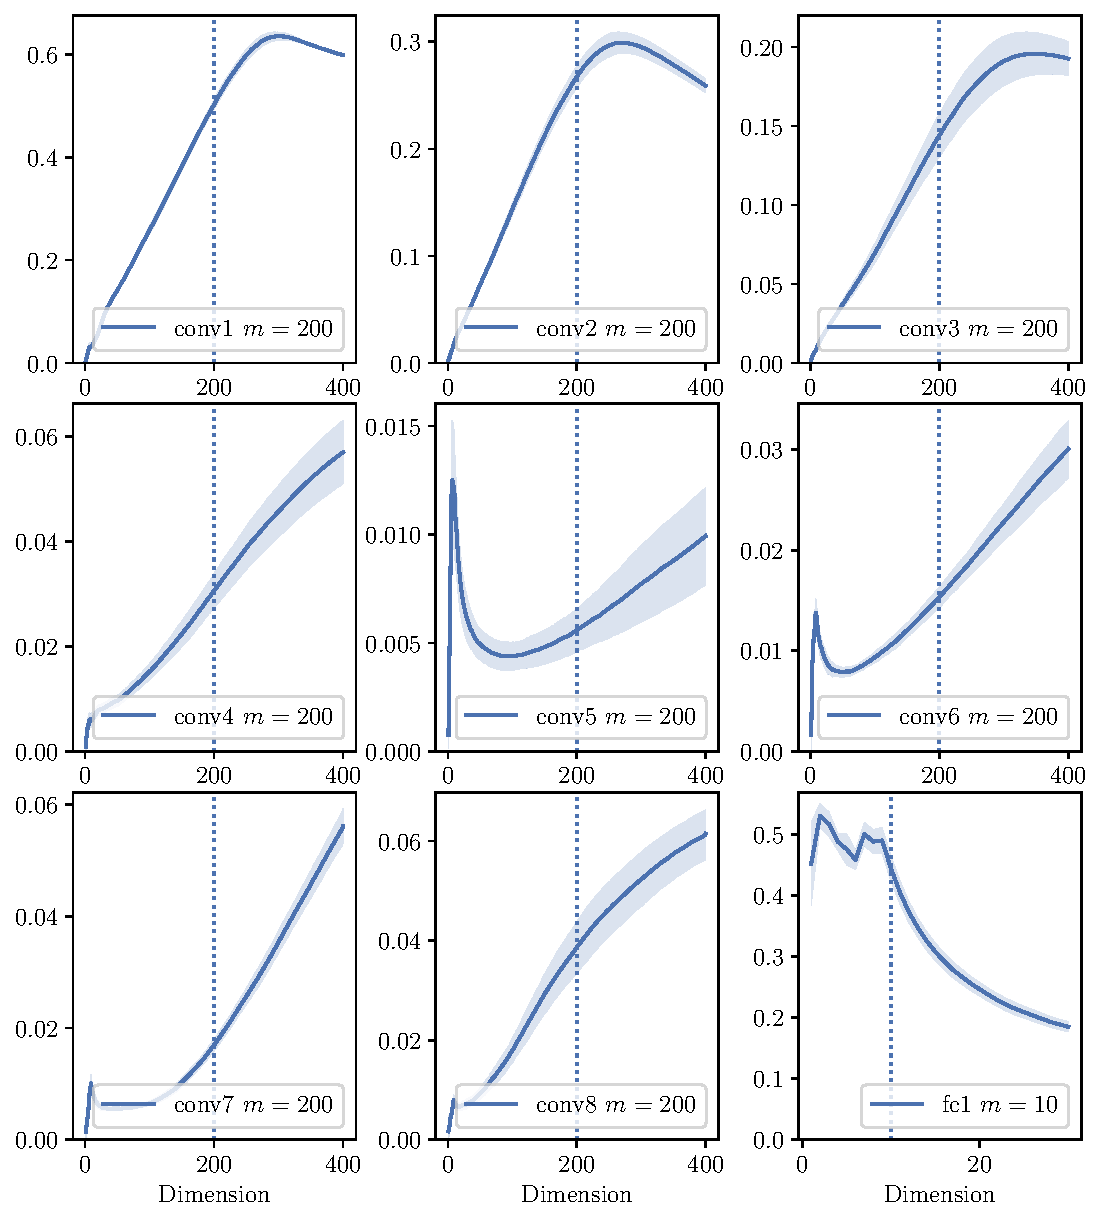
\includegraphics[width=0.48\textwidth]{Appendix_Figures/Overlap_large_model/overlap_raw/DimOverlap_CIFAR10_VGG11W200_fxlr0.01_appendix_vertical_3col.pdf}}\\
%     \subfigure[\centering\small{VGG11-W200 (CIFAR10)}]{
%     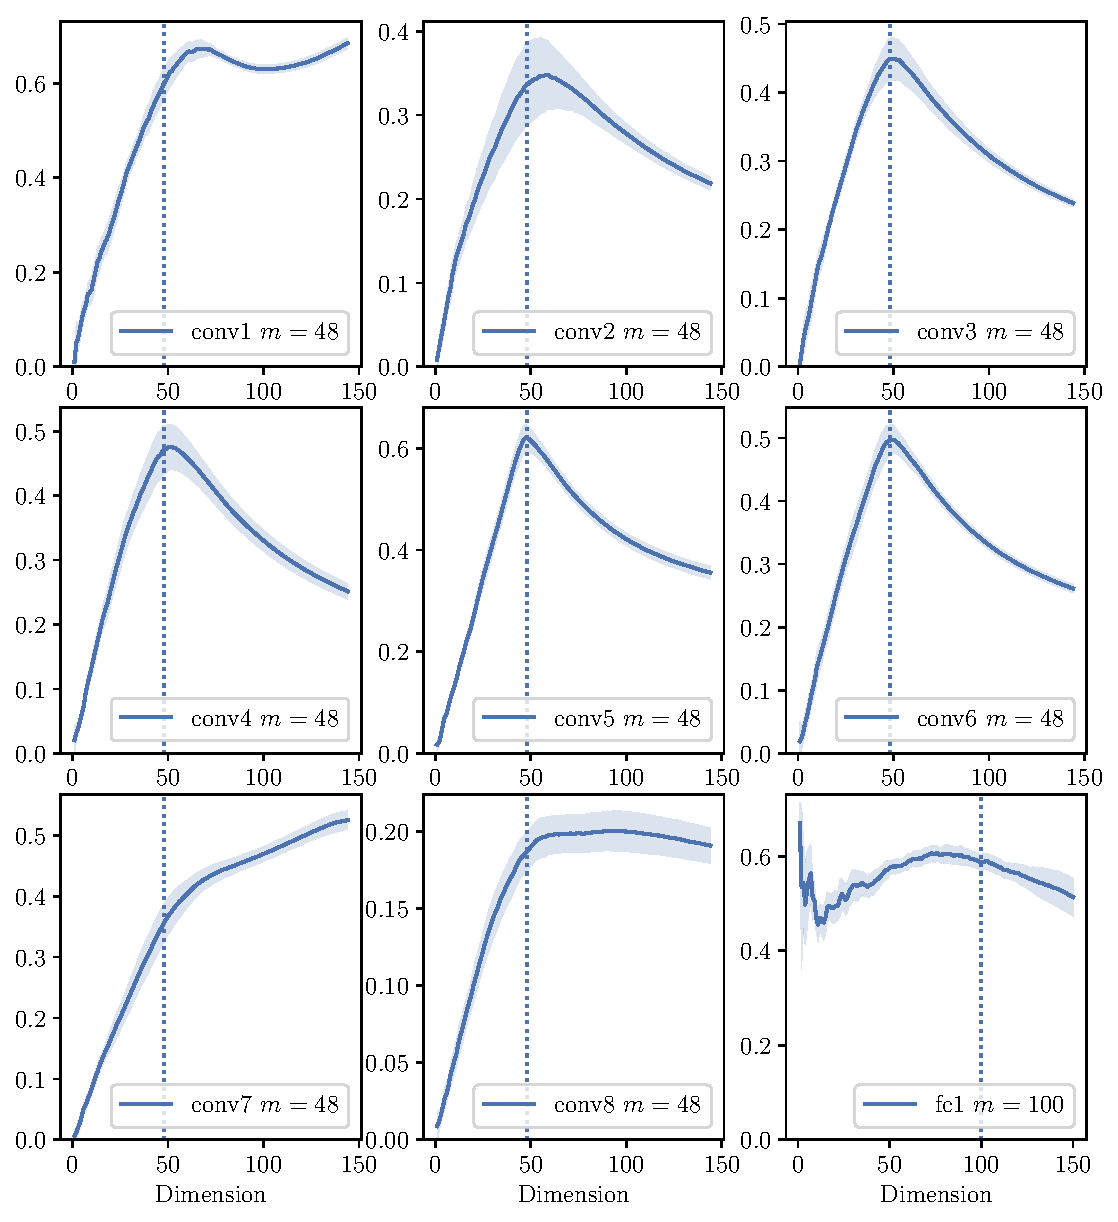
\includegraphics[width=0.48\textwidth]{Appendix_Figures/Overlap_large_model/overlap_raw/DimOverlap_CIFAR100_VGG11W48New_nobn_fixlr0.01_appendix_vertical_3col.pdf}}
%     \subfigure[\centering\small{VGG11-W80 (CIFAR100)}]{
%     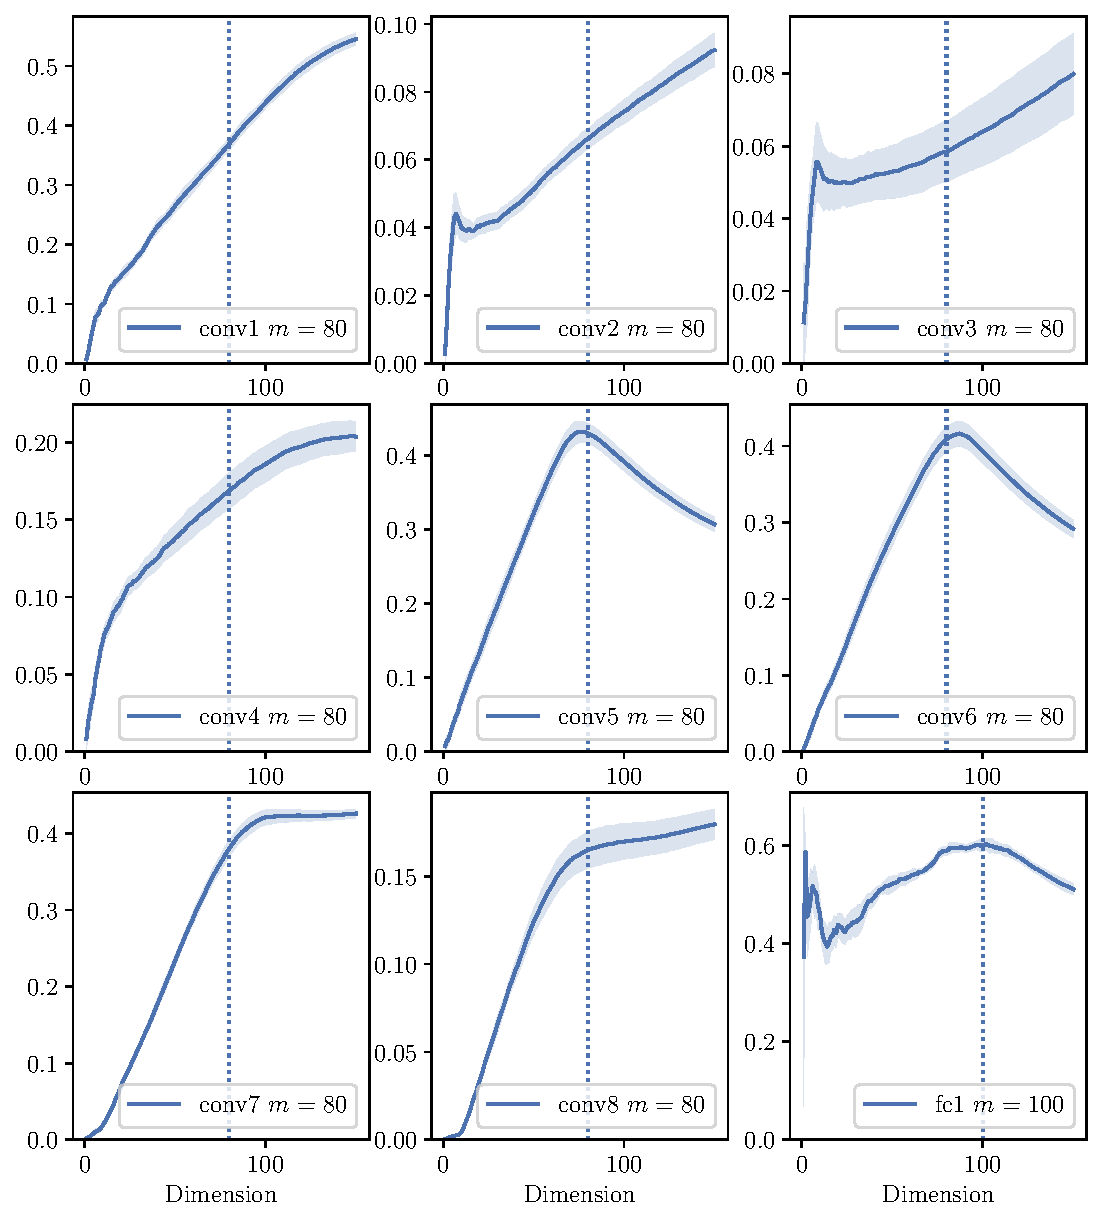
\includegraphics[width=0.48\textwidth]{Appendix_Figures/Overlap_large_model/overlap_raw/DimOverlap_CIFAR100_VGG11W80New_nobn_fixlr0.01_appendix_vertical_3col.pdf}}
%     \caption{Top Eigenspace overlap for varients of VGG11 on CIFAR10 and CIFAR100.}
%     \label{fig:app_adexp_vgg}
% \end{figure}

\begin{figure}[H]
    \centering
    \begin{subfigure}[b]{0.48\textwidth}
        \centering
        \captionsetup{justification=centering}
        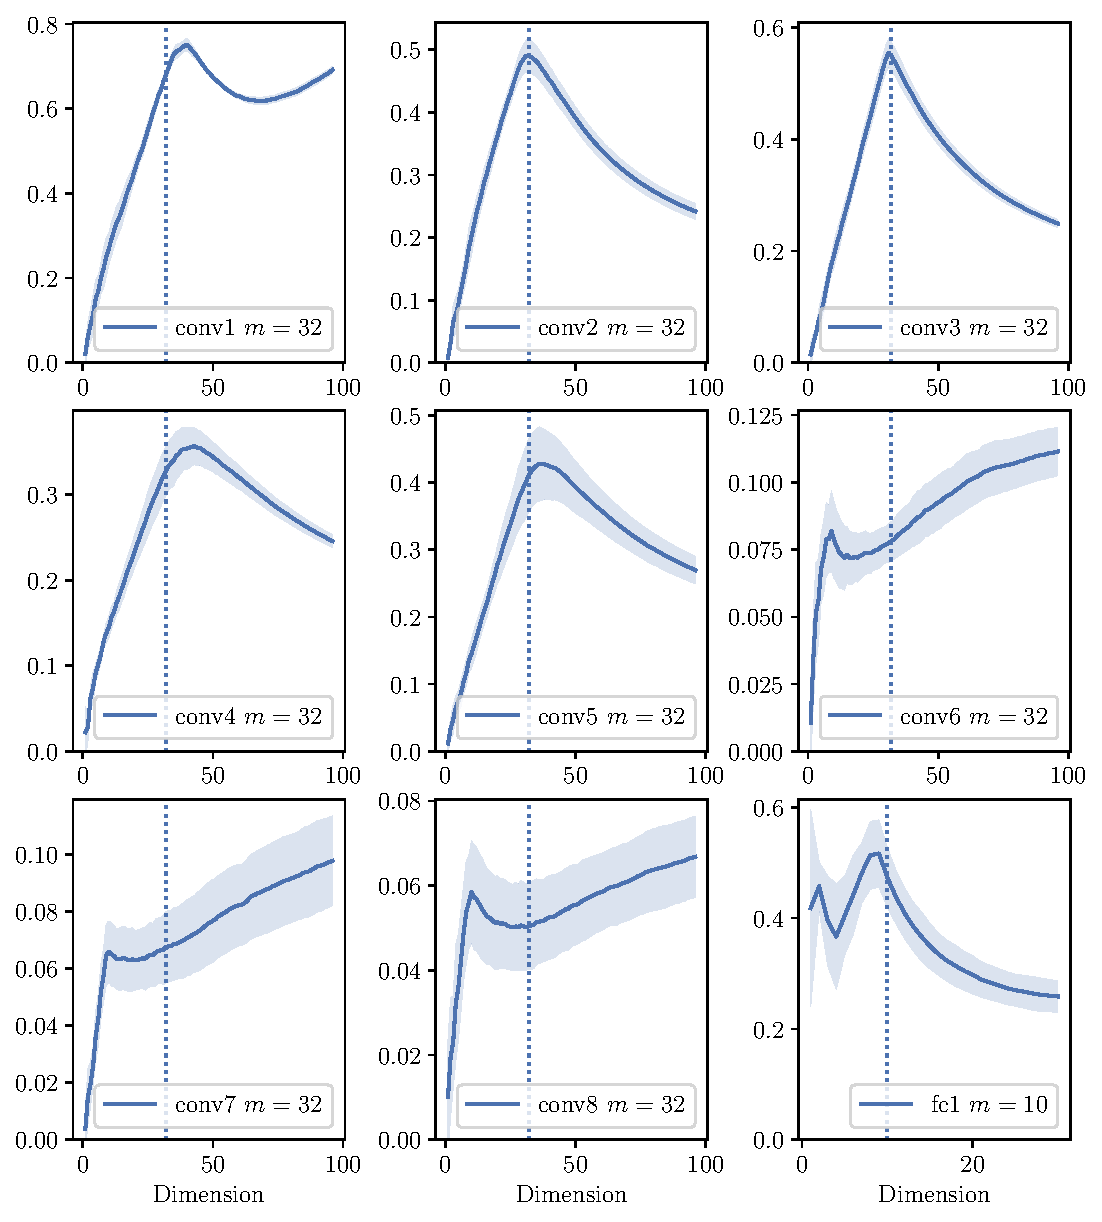
\includegraphics[width=\textwidth]{Appendix_Figures/Overlap_large_model/overlap_raw/DimOverlap_CIFAR10_VGG11W32_fixlr0.01_appendix_vertical_3col.pdf}
        \caption{VGG11-W32 (CIFAR10)}
        \label{fig:app_adexp_cifar10_vgg32}
    \end{subfigure}%
    \ \ \ \ \ \
    \begin{subfigure}[b]{0.48\textwidth}
        \centering
        \captionsetup{justification=centering}
        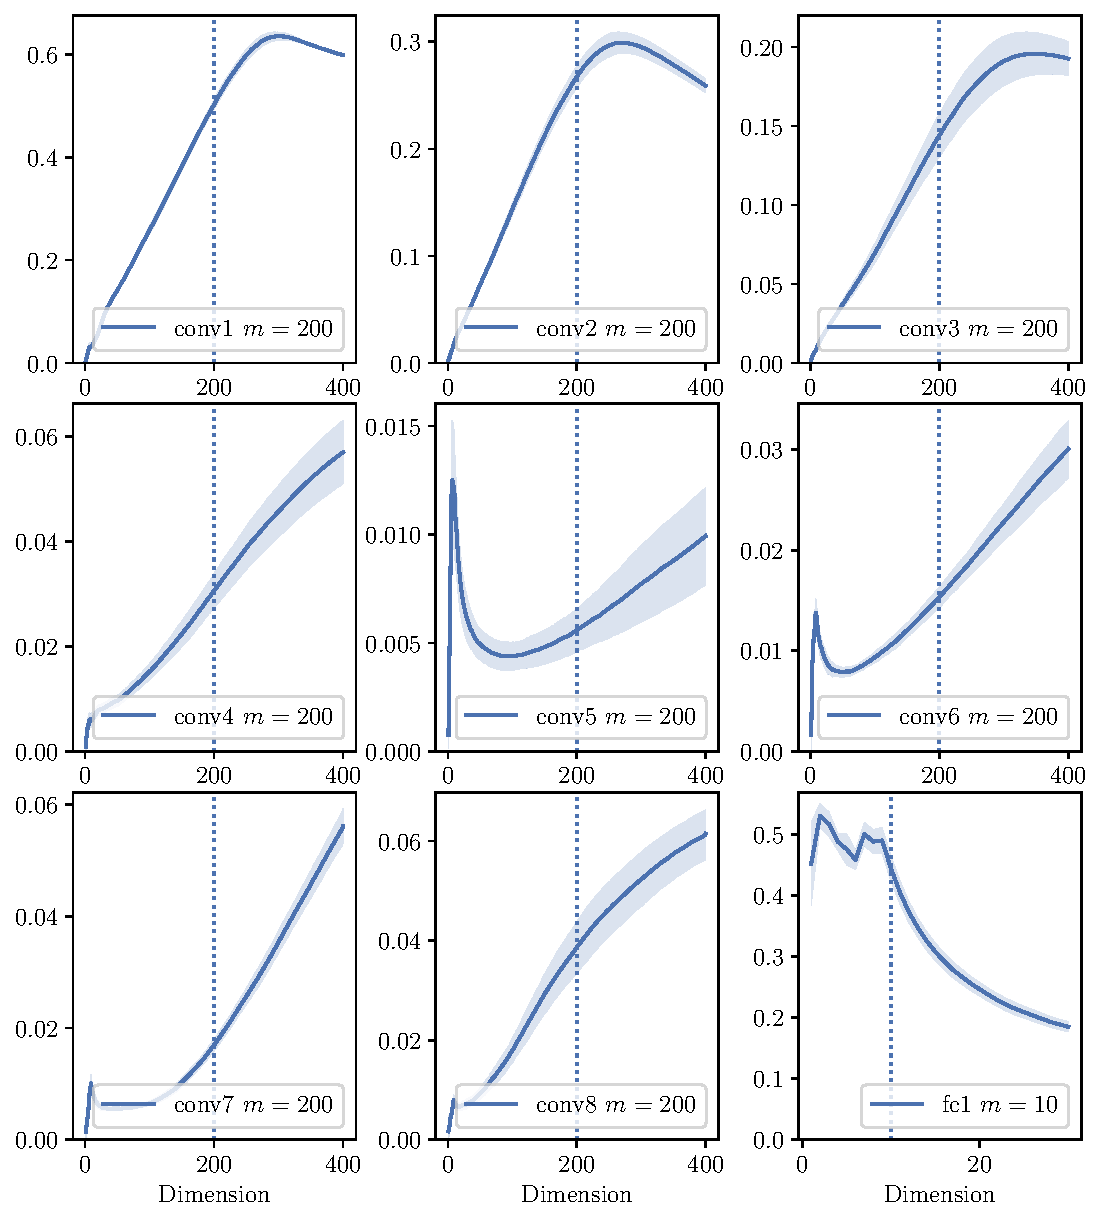
\includegraphics[width=\textwidth]{Appendix_Figures/Overlap_large_model/overlap_raw/DimOverlap_CIFAR10_VGG11W200_fxlr0.01_appendix_vertical_3col.pdf}
        \caption{VGG11-W200 (CIFAR10)}
        \label{fig:app_adexp_cifar10_vgg200}
    \end{subfigure}
    \\\vspace{0.1in}
    \begin{subfigure}[b]{0.48\textwidth}
        \centering
        \captionsetup{justification=centering}
        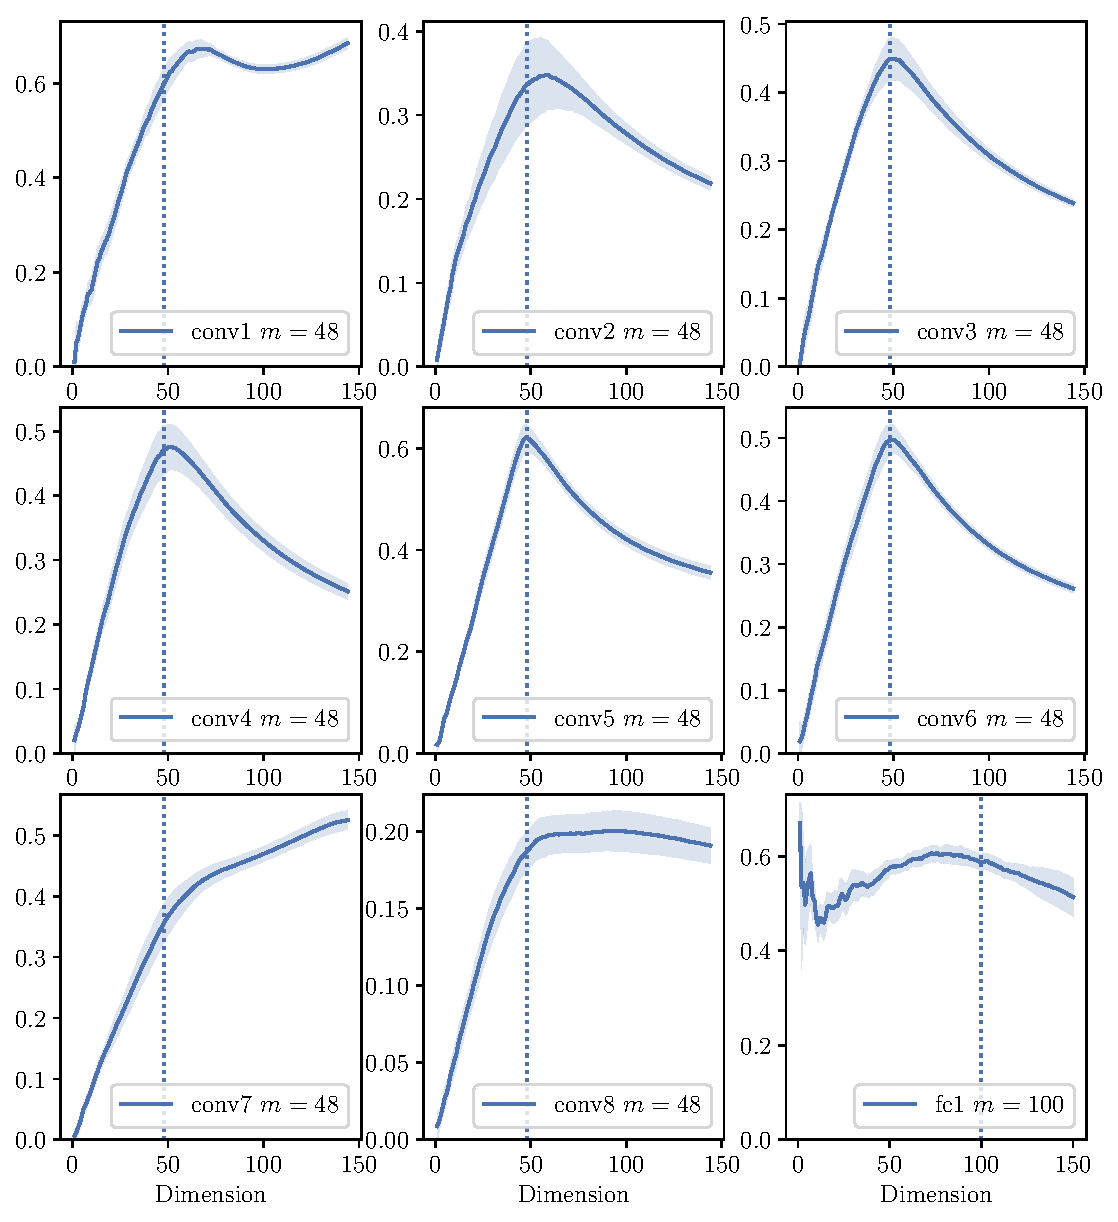
\includegraphics[width=\textwidth]{Appendix_Figures/Overlap_large_model/overlap_raw/DimOverlap_CIFAR100_VGG11W48New_nobn_fixlr0.01_appendix_vertical_3col.pdf}
        \caption{VGG11-W48 (CIFAR100)}
        \label{fig:app_adexp_cifar100_vgg48}
    \end{subfigure}%
    \ \ \ \ \ \
    \begin{subfigure}[b]{0.48\textwidth}
        \centering
        \captionsetup{justification=centering}
        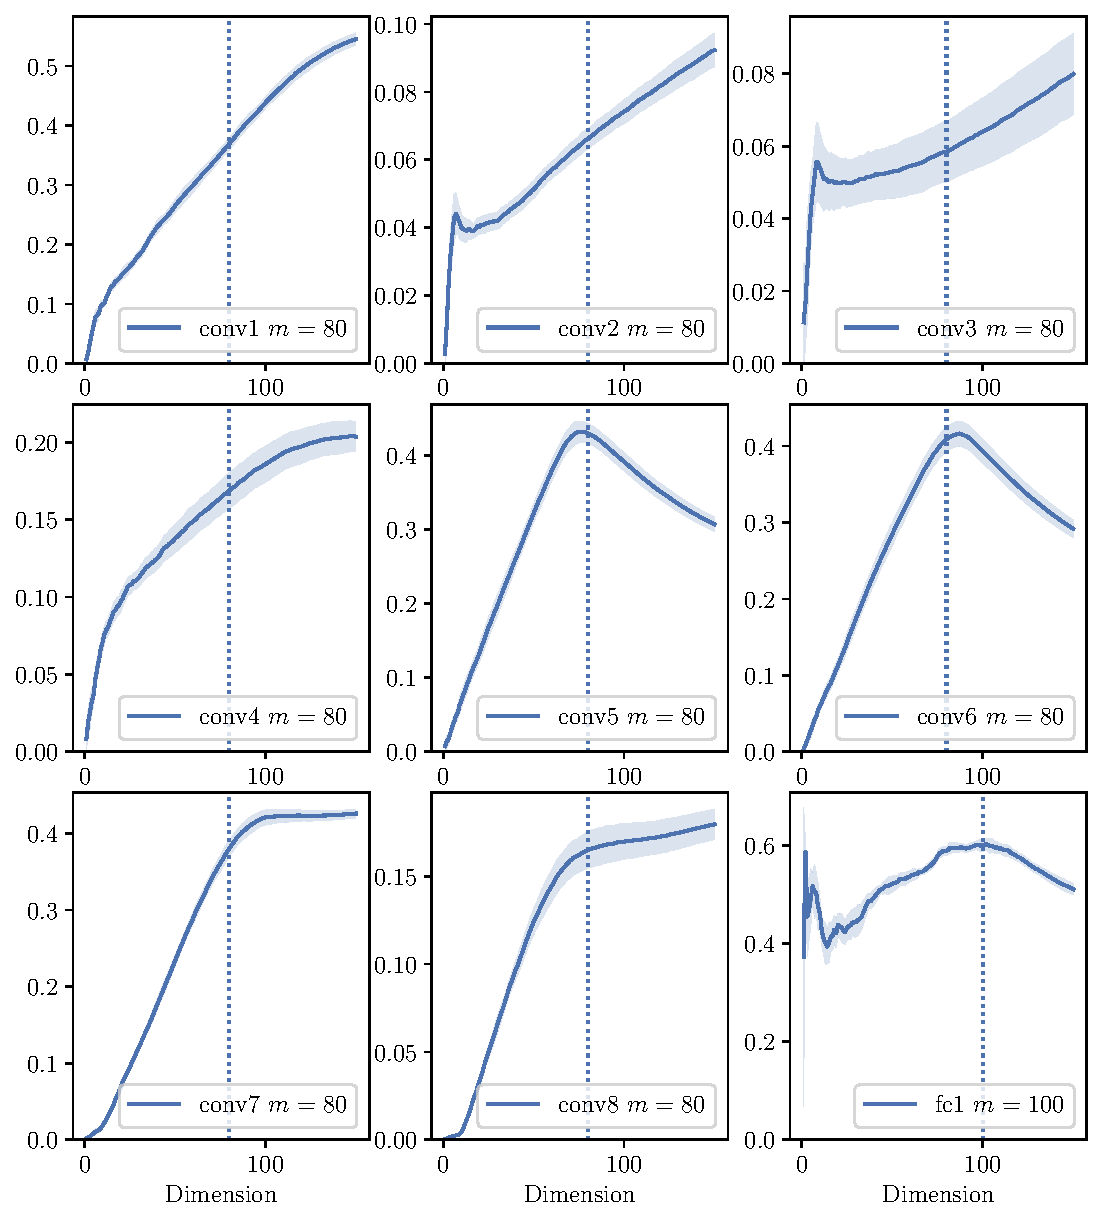
\includegraphics[width=\textwidth]{Appendix_Figures/Overlap_large_model/overlap_raw/DimOverlap_CIFAR100_VGG11W80New_nobn_fixlr0.01_appendix_vertical_3col.pdf}
        \caption{VGG11-W80 (CIFAR100)}
        \label{fig:app_adexp_cifar100_vgg80}
    \end{subfigure}
    \captionsetup{justification=centering}
    \caption{Top Eigenspace overlap for varients of VGG11 on CIFAR10 and CIFAR100}
    \label{fig:app_adexp_vgg}
\end{figure}

% \begin{figure}[H]
%     \centering
%     \subfigure[\centering\small{ResNet18-W48 (CIFAR100)}]{
%     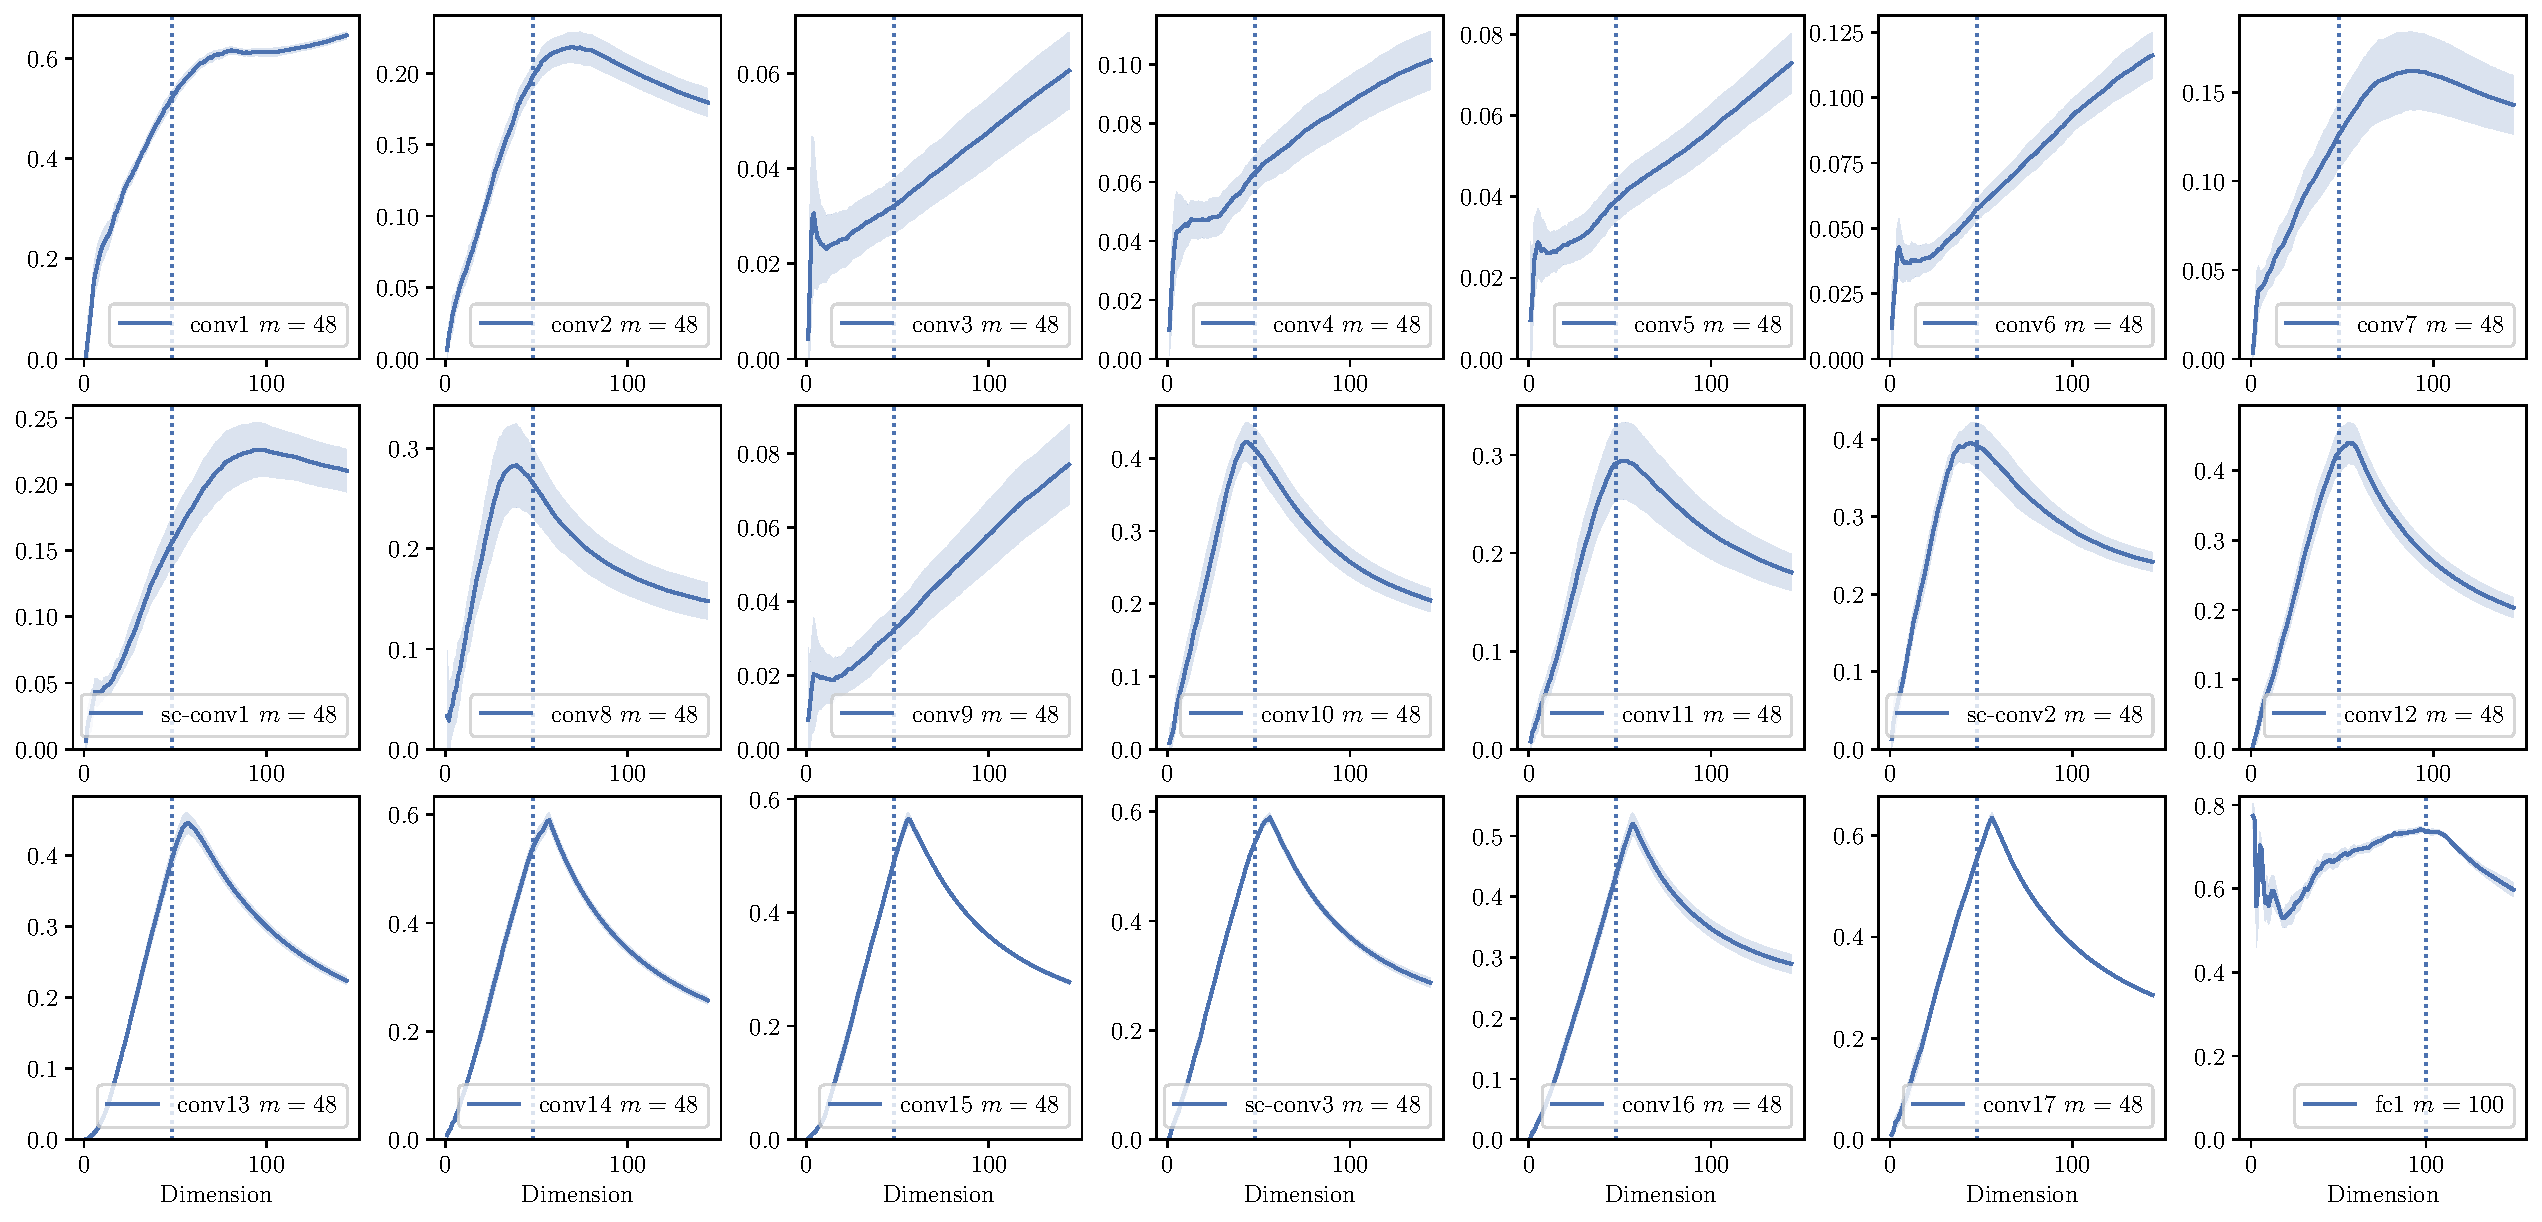
\includegraphics[width=0.8\textwidth]{Appendix_Figures/Overlap_large_model/overlap_raw/ResNet/Resnet18W48New_nobn_fixlr0.01_appendix_vertical_7col.pdf}}\\
%     \subfigure[\centering\small{ResNet18-W64 (CIFAR100)}]{
%     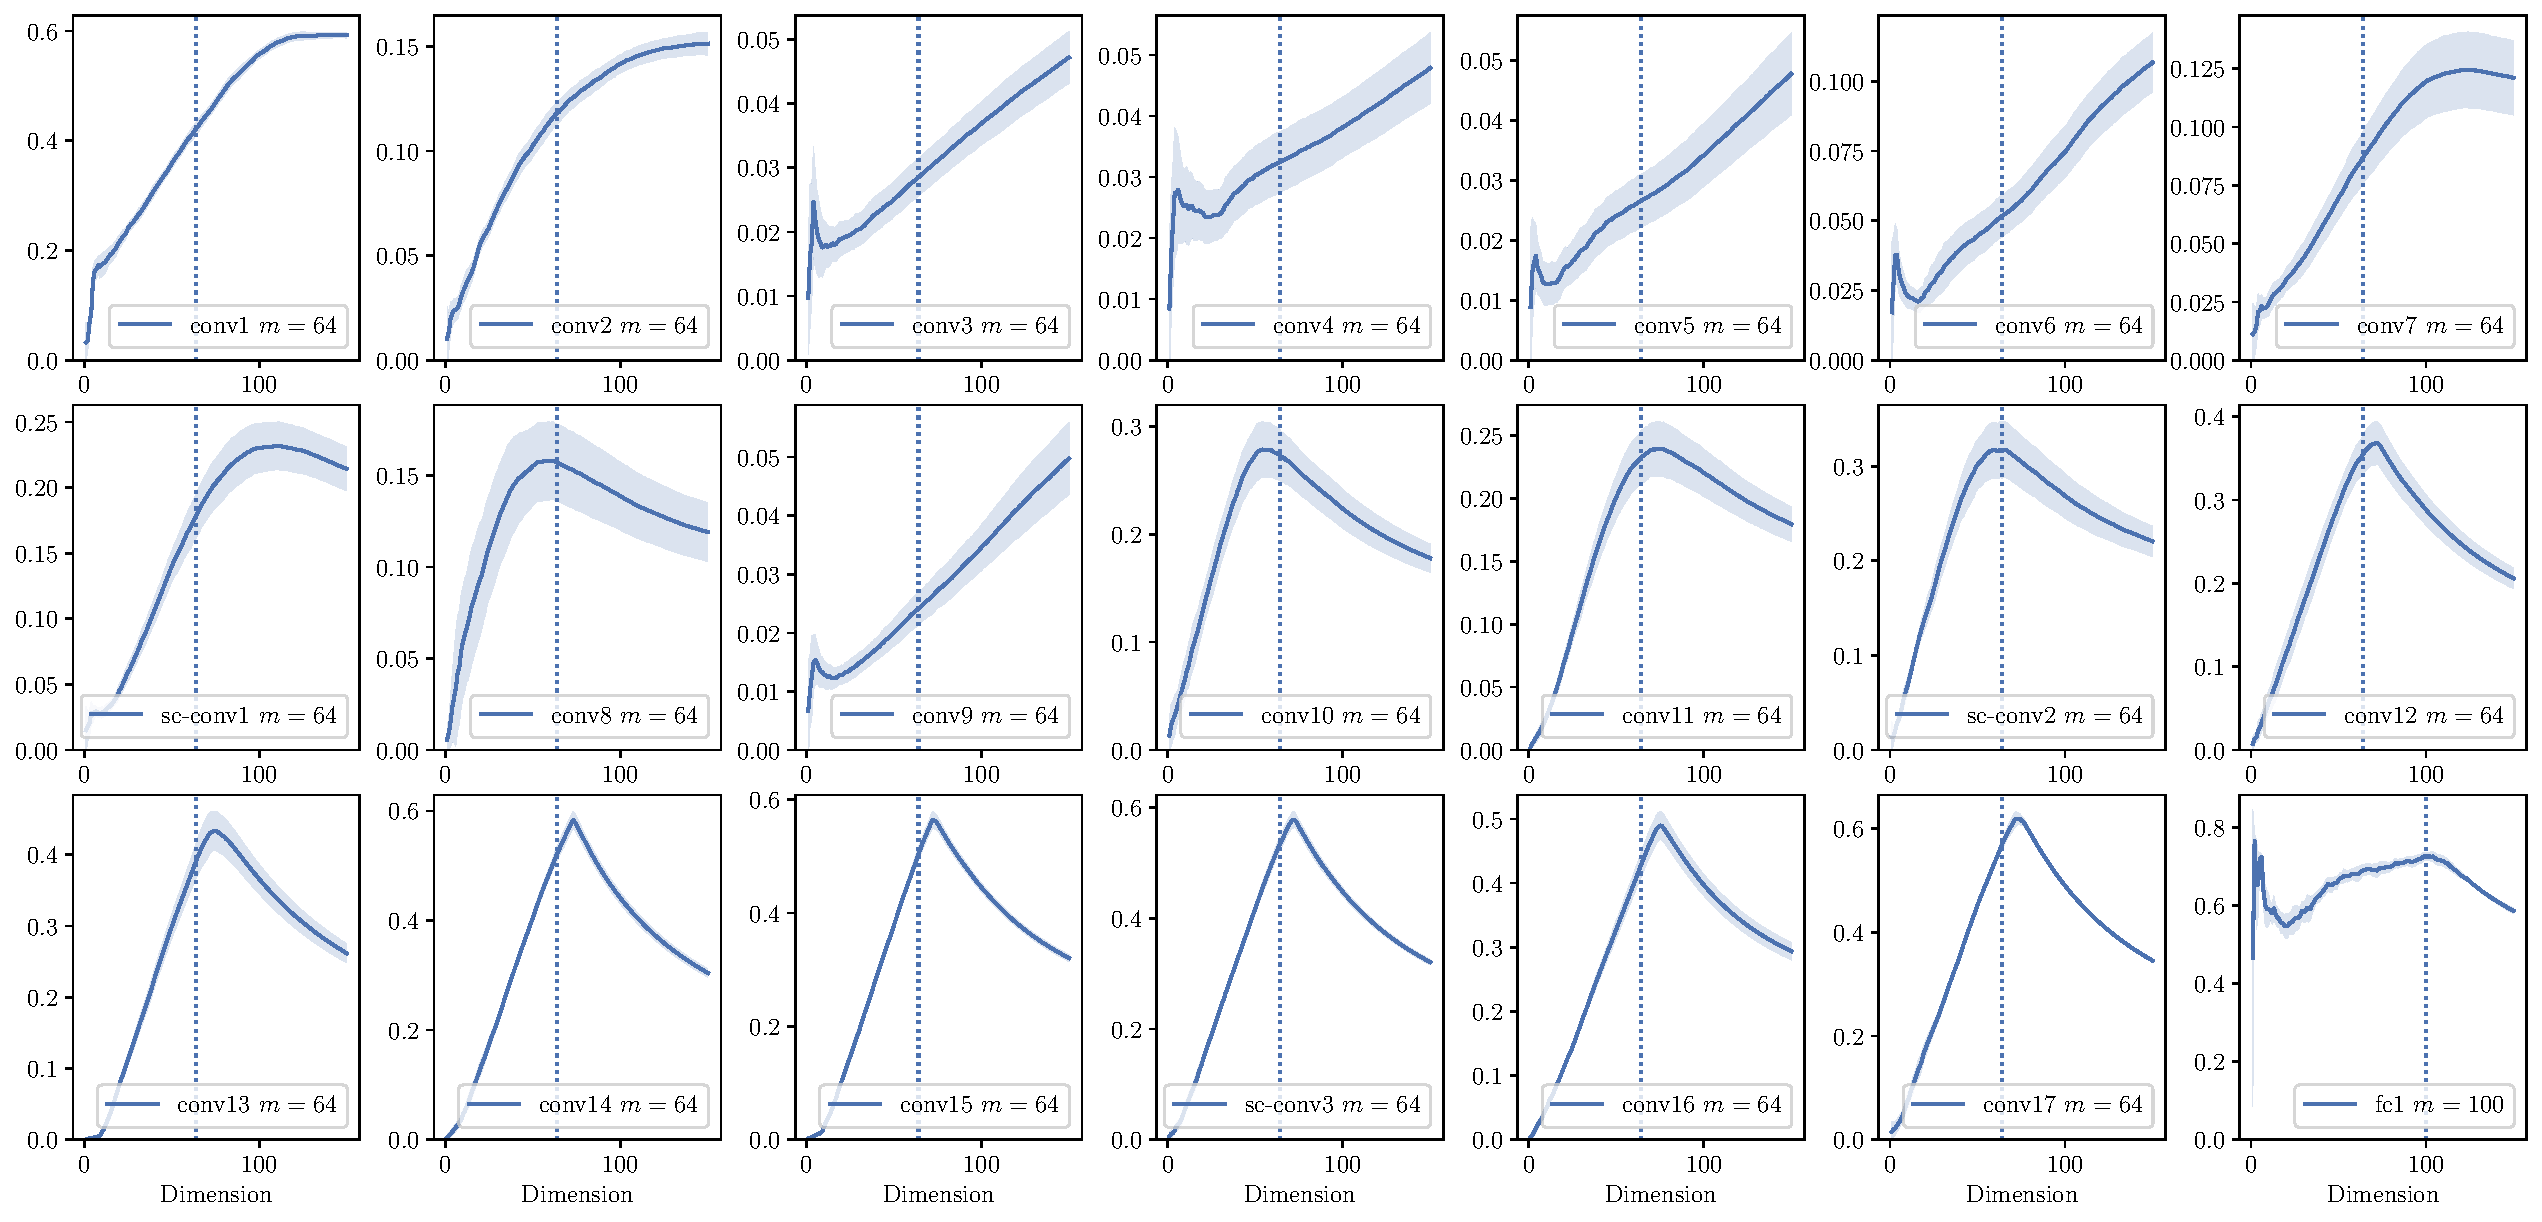
\includegraphics[width=0.8\textwidth]{Appendix_Figures/Overlap_large_model/overlap_raw/ResNet/Resnet18W64New_nobn_fixlr0.01_appendix_vertical_7col.pdf}}\\
%     \subfigure[\centering\small{ResNet18-W80 (CIFAR100)}]{
%     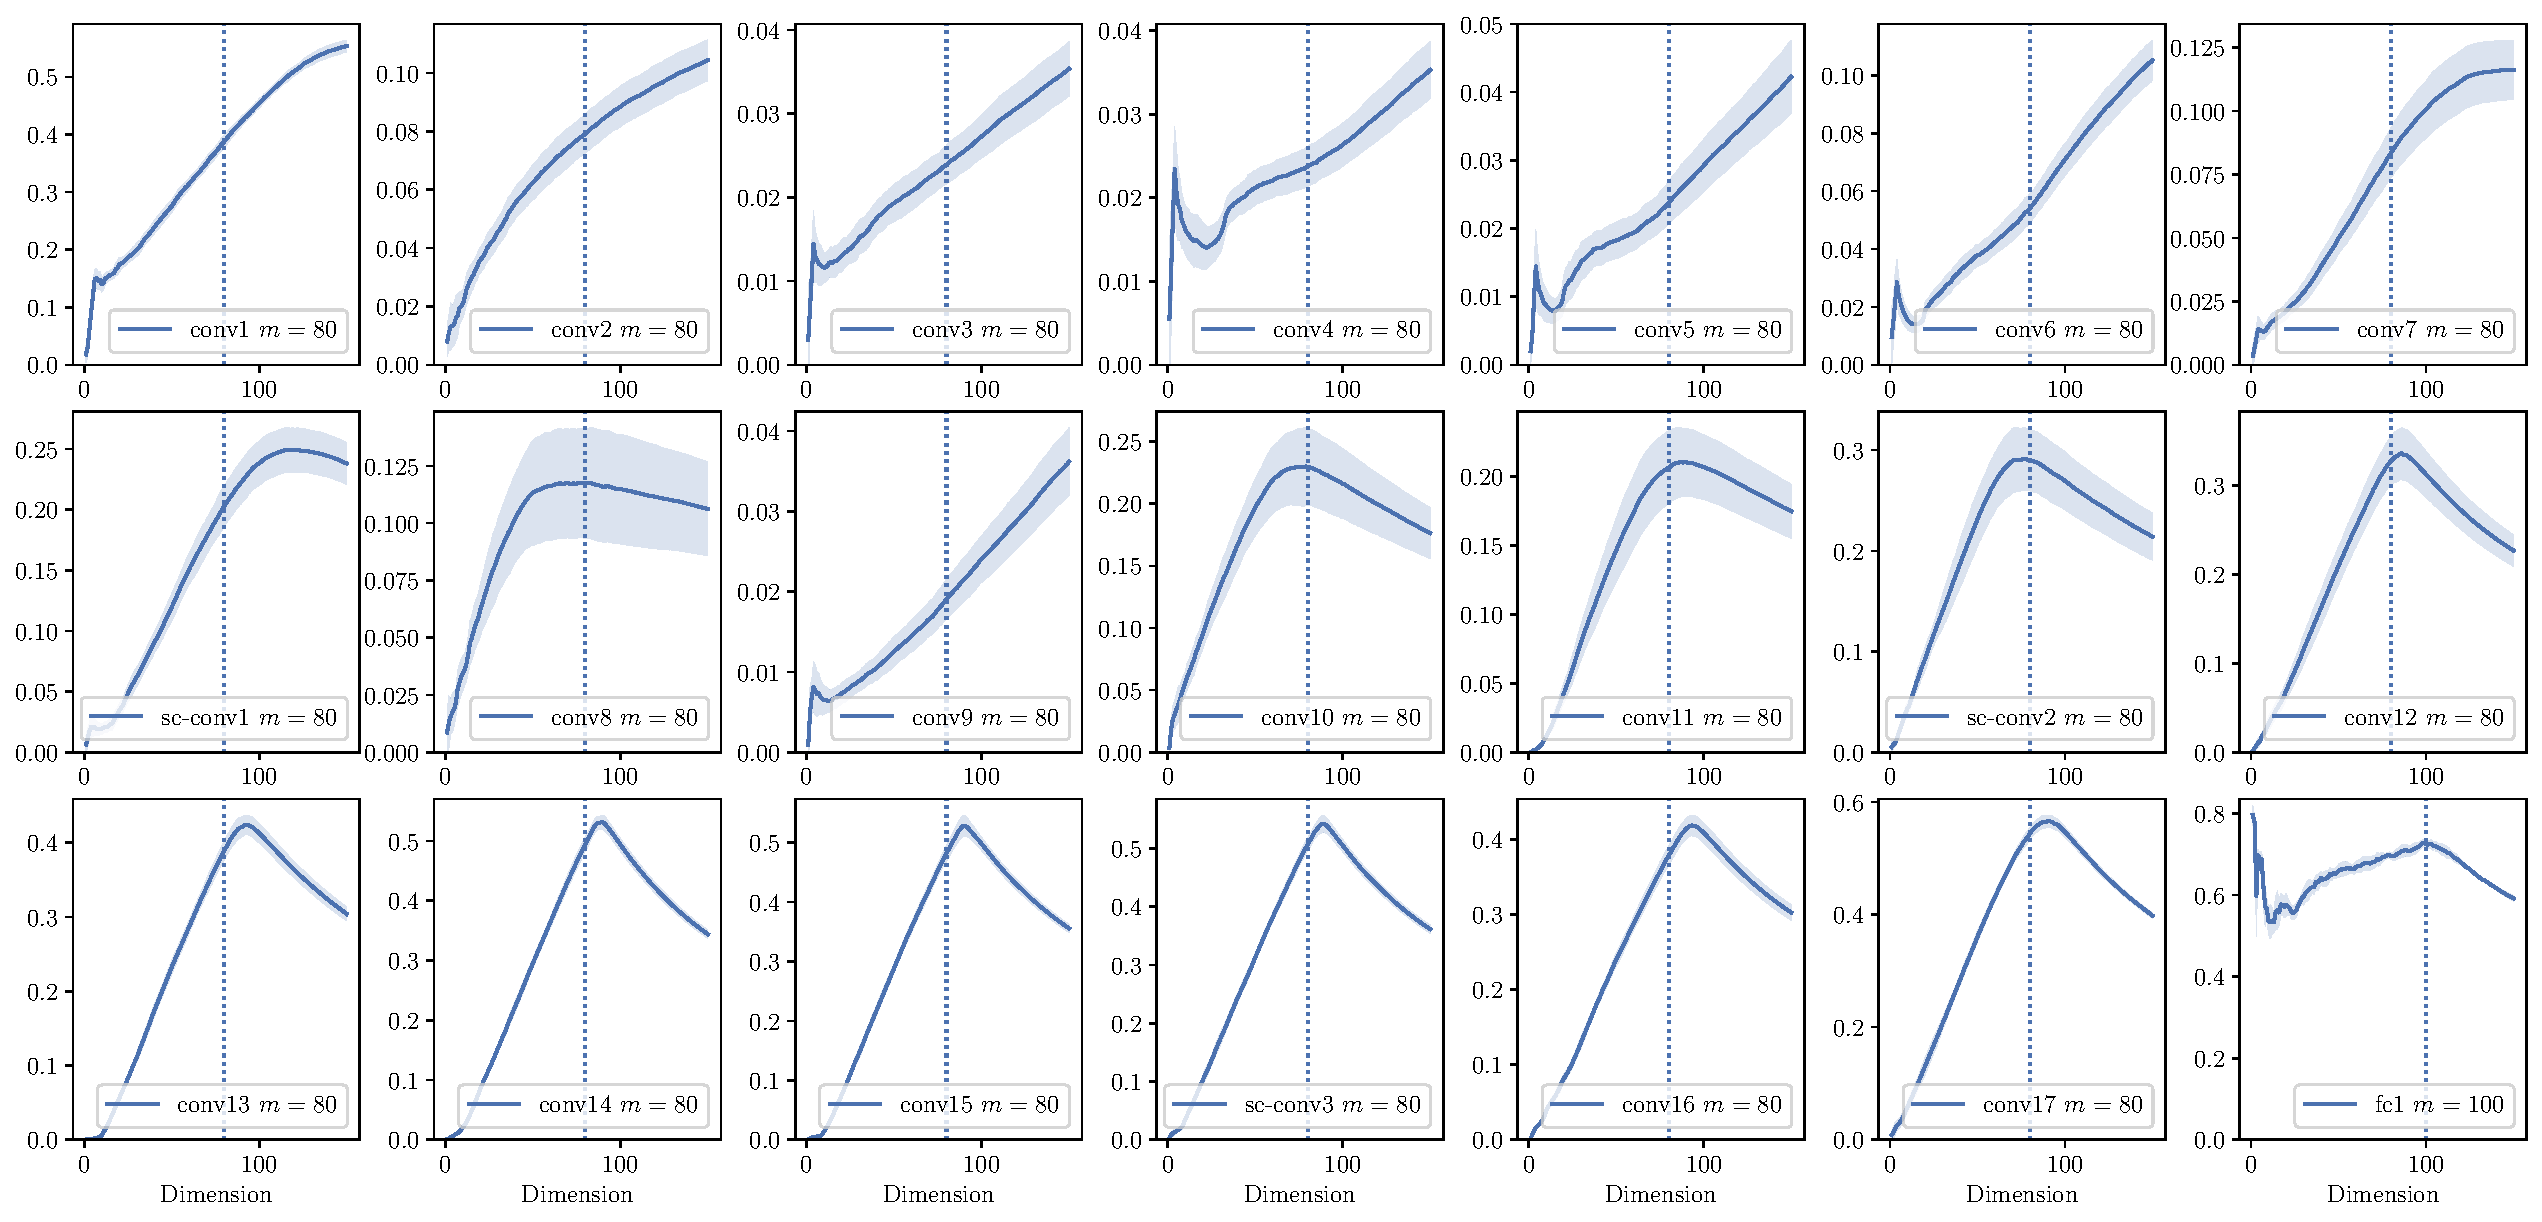
\includegraphics[width=0.8\textwidth]{Appendix_Figures/Overlap_large_model/overlap_raw/ResNet/Resnet18W80_nobn_fixlr0.01_appendix_vertical_7col.pdf}}
%     \caption{Top Eigenspace overlap for variants of ResNet18 on CIFAR100}
%     \label{fig:app_adexp_resnet}
% \end{figure}

\begin{figure}[H]
    \centering
    \begin{subfigure}[b]{\textwidth}
        \centering
        \captionsetup{justification=centering}
        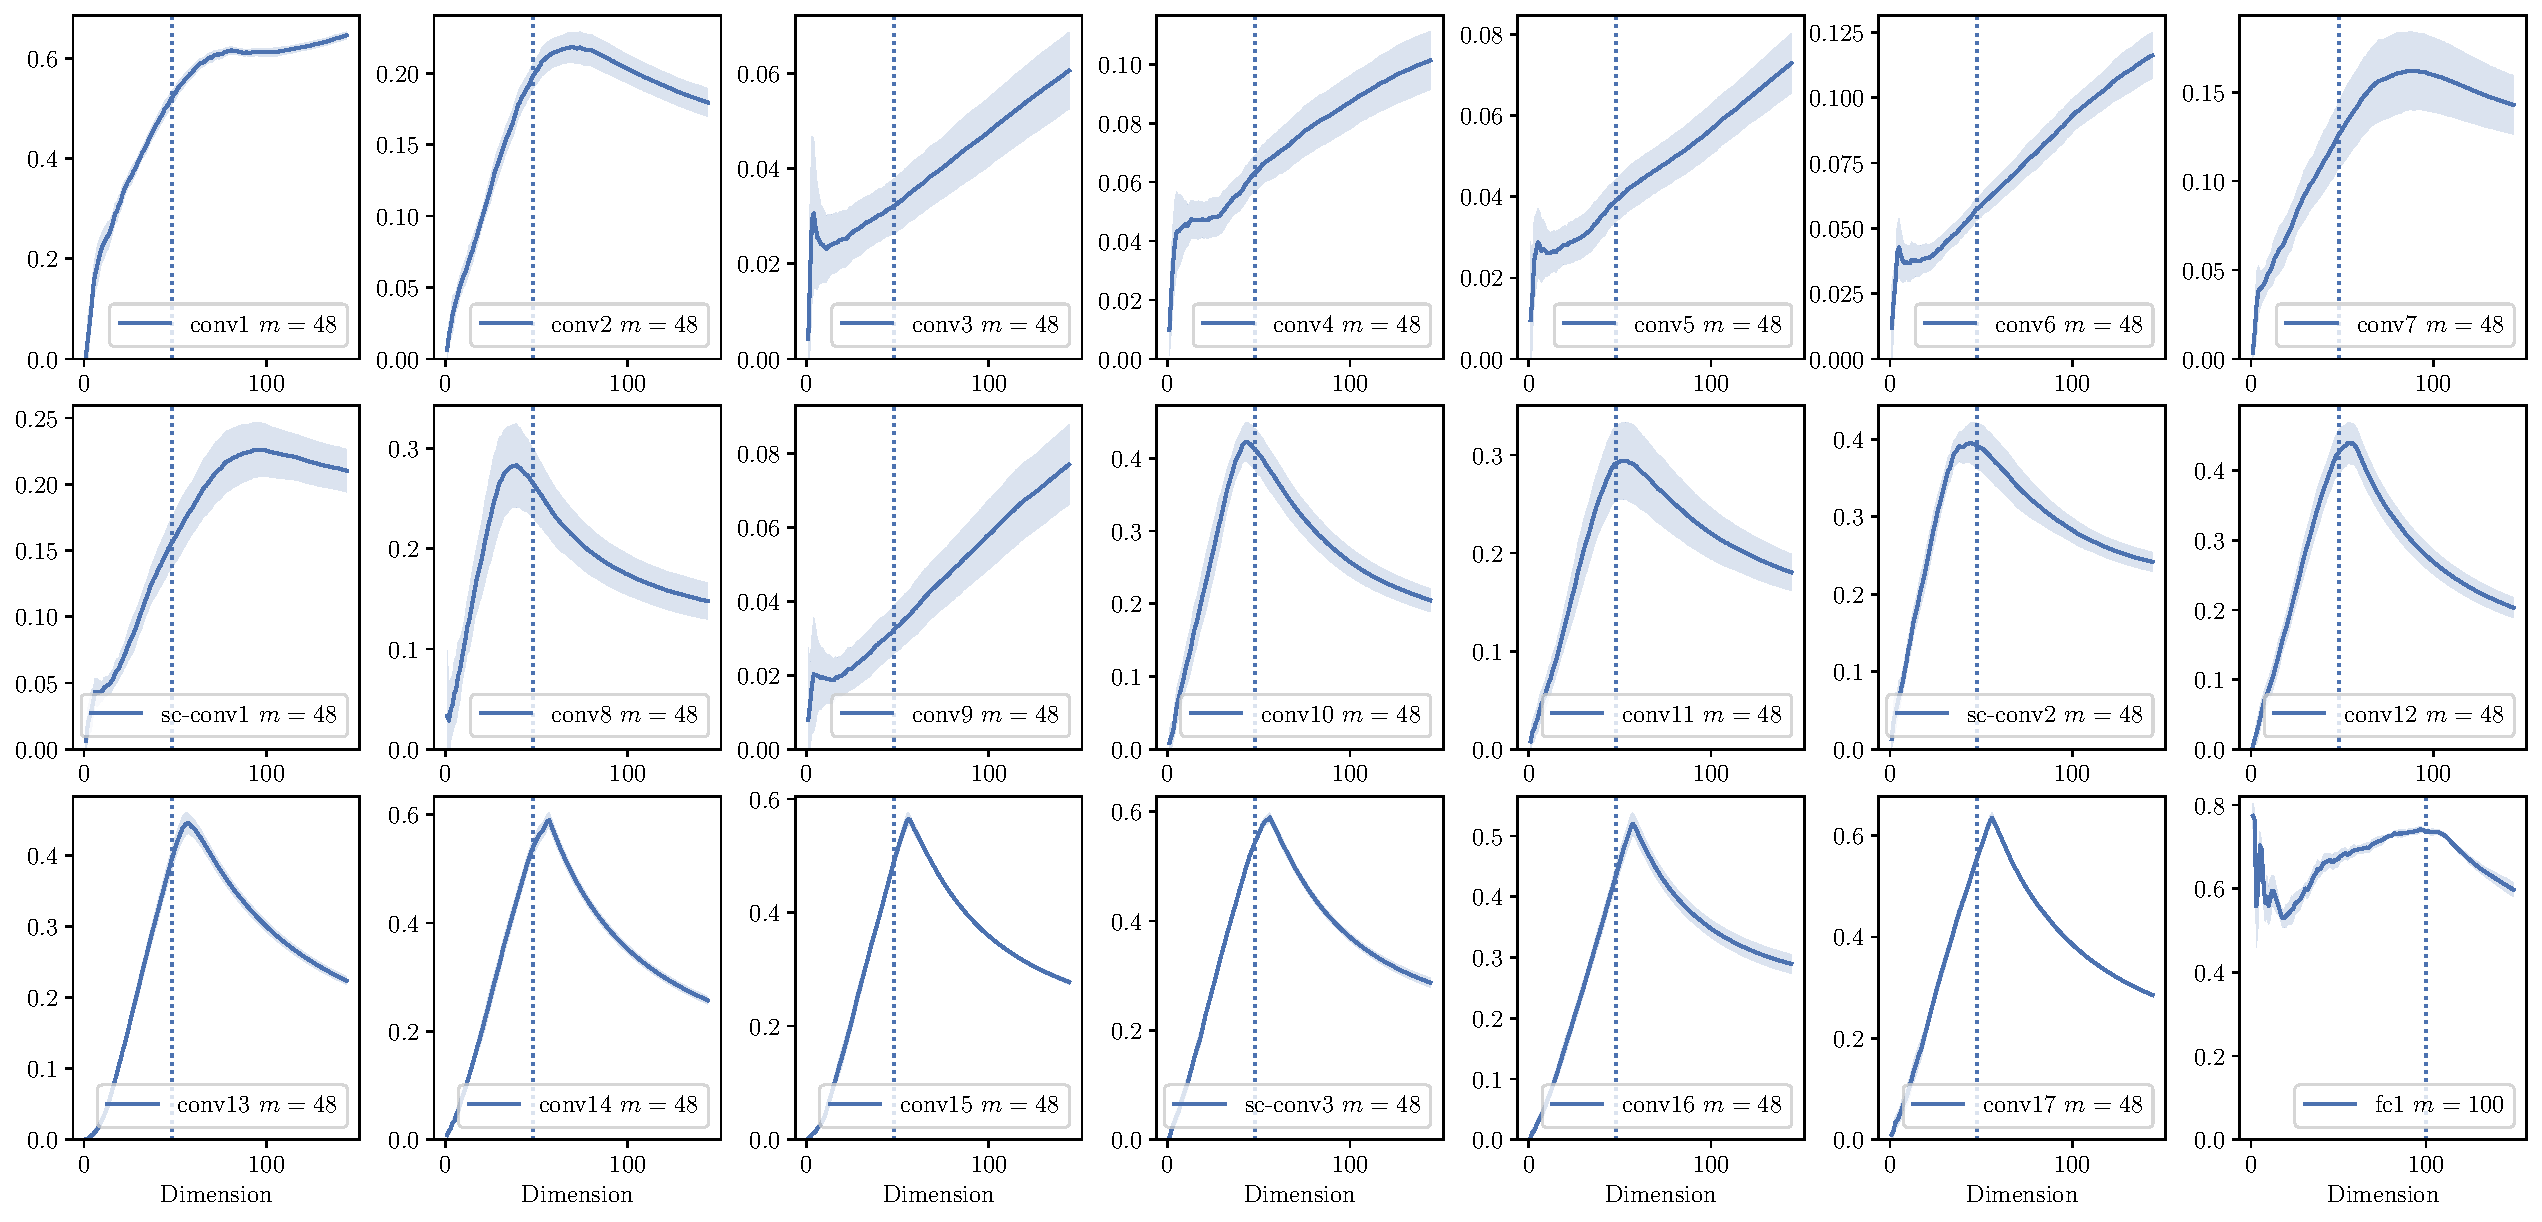
\includegraphics[width=\textwidth]{Appendix_Figures/Overlap_large_model/overlap_raw/ResNet/Resnet18W48New_nobn_fixlr0.01_appendix_vertical_7col.pdf}
        \caption{ResNet18-W48 (CIFAR100)}
        \label{fig:app_adexp_cifar100_resnet48}
    \end{subfigure}%
    \\
    \begin{subfigure}[b]{\textwidth}
        \centering
        \captionsetup{justification=centering}
        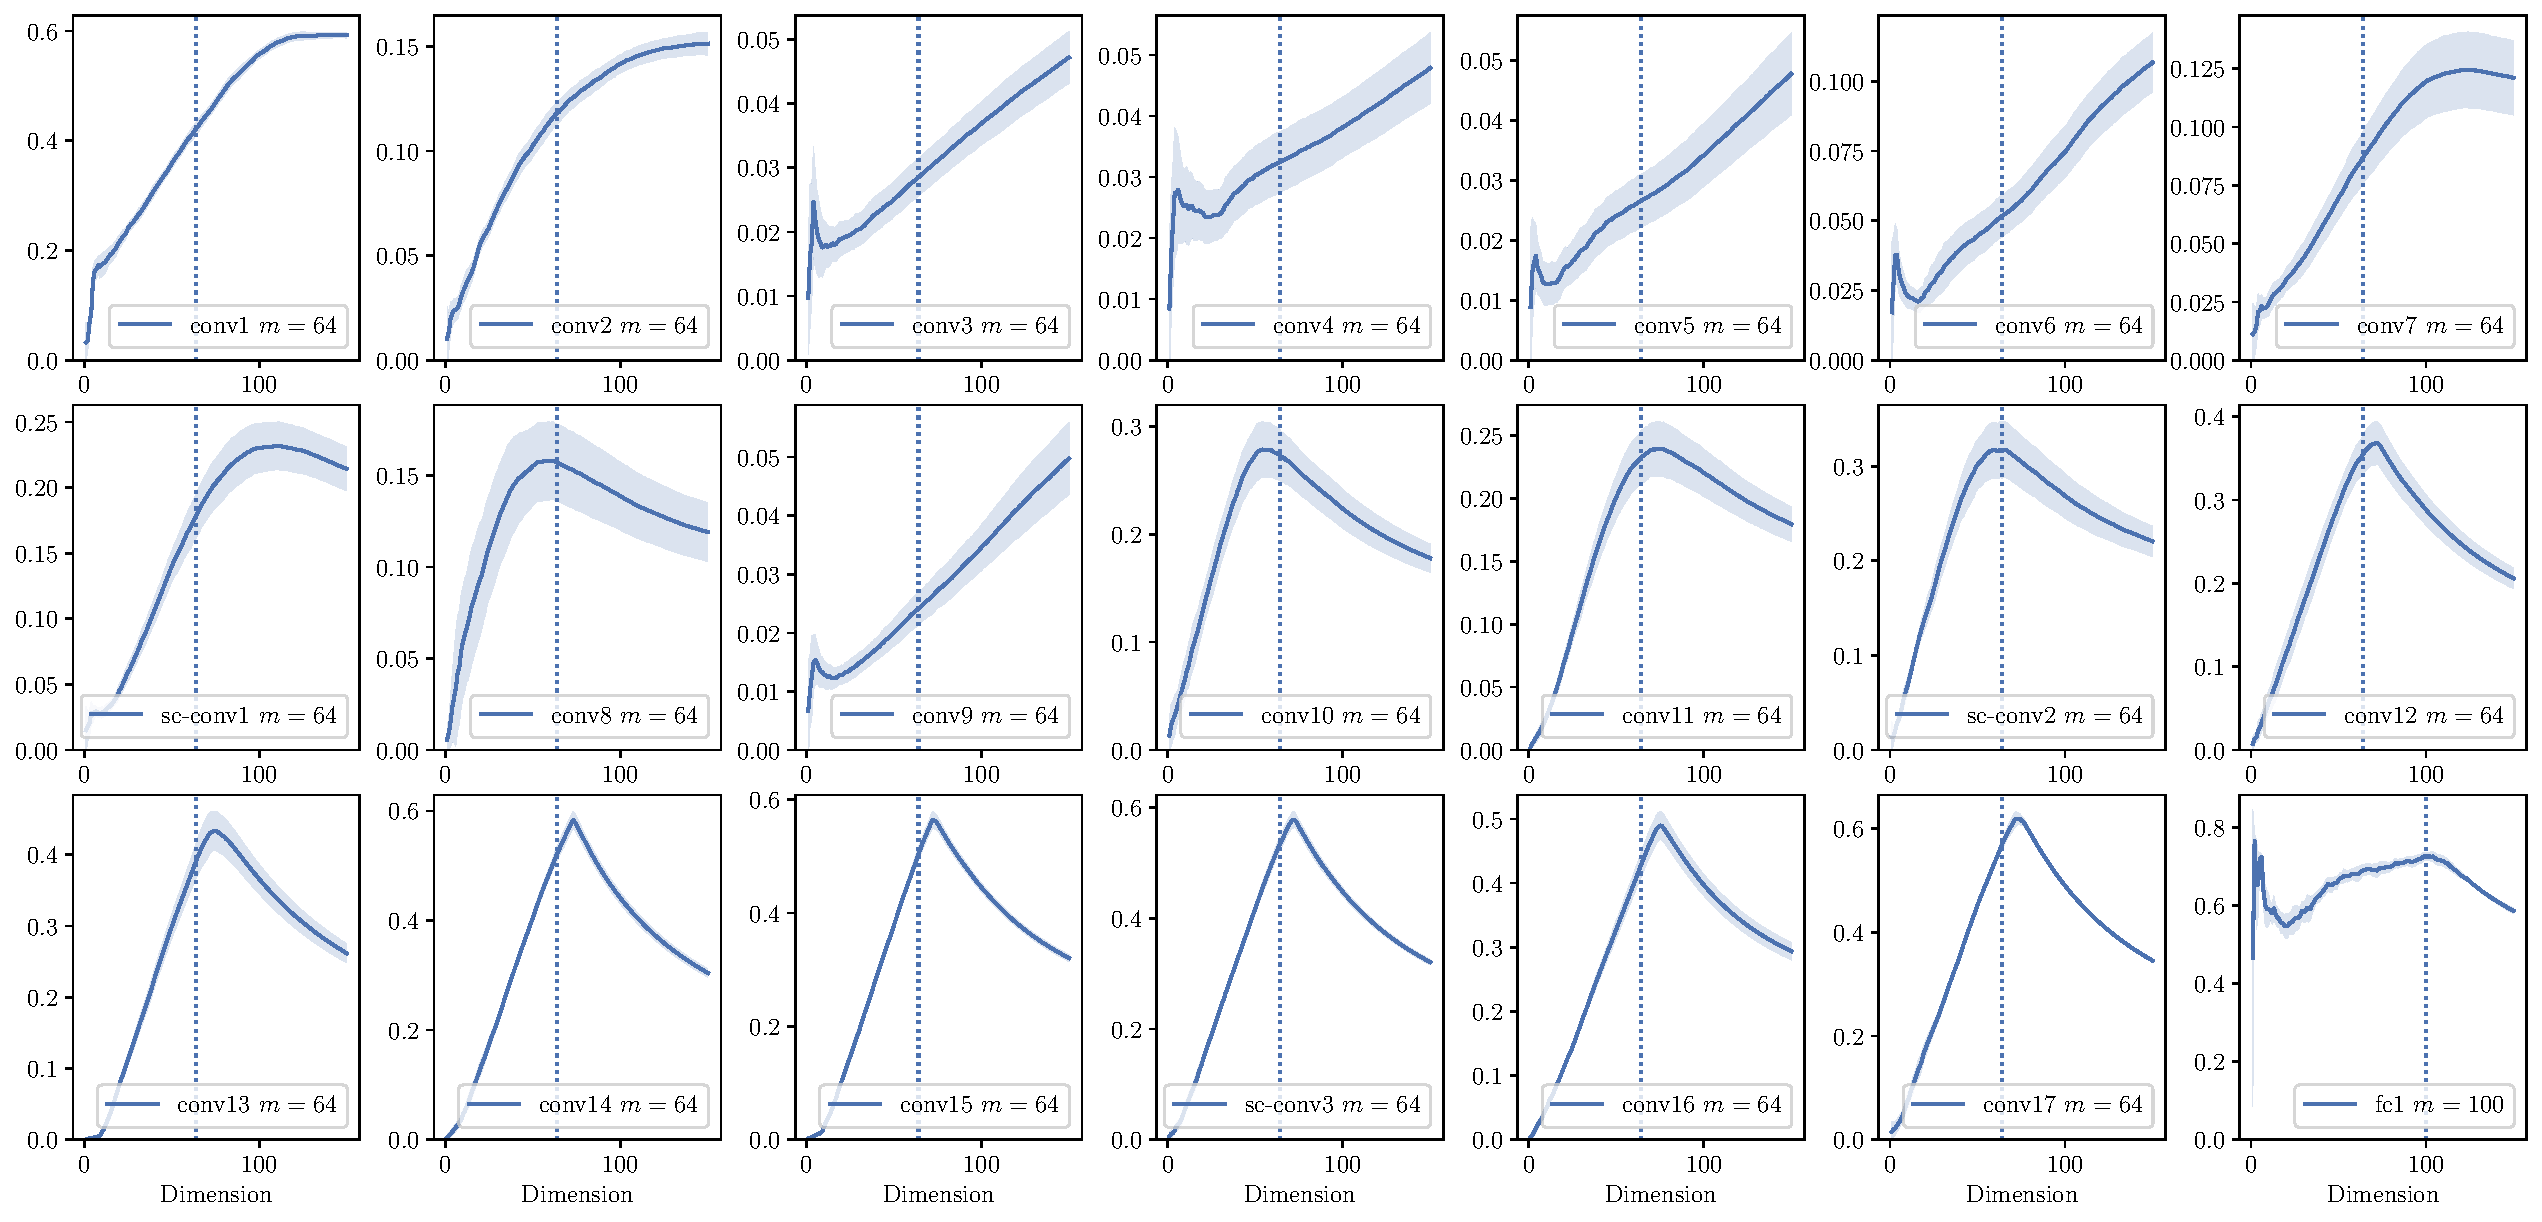
\includegraphics[width=\textwidth]{Appendix_Figures/Overlap_large_model/overlap_raw/ResNet/Resnet18W64New_nobn_fixlr0.01_appendix_vertical_7col.pdf}
        \caption{ResNet18-W64 (CIFAR100)}
        \label{fig:app_adexp_cifar100_resnet64}
    \end{subfigure}
    \\
    \begin{subfigure}[b]{\textwidth}
        \centering
        \captionsetup{justification=centering}
        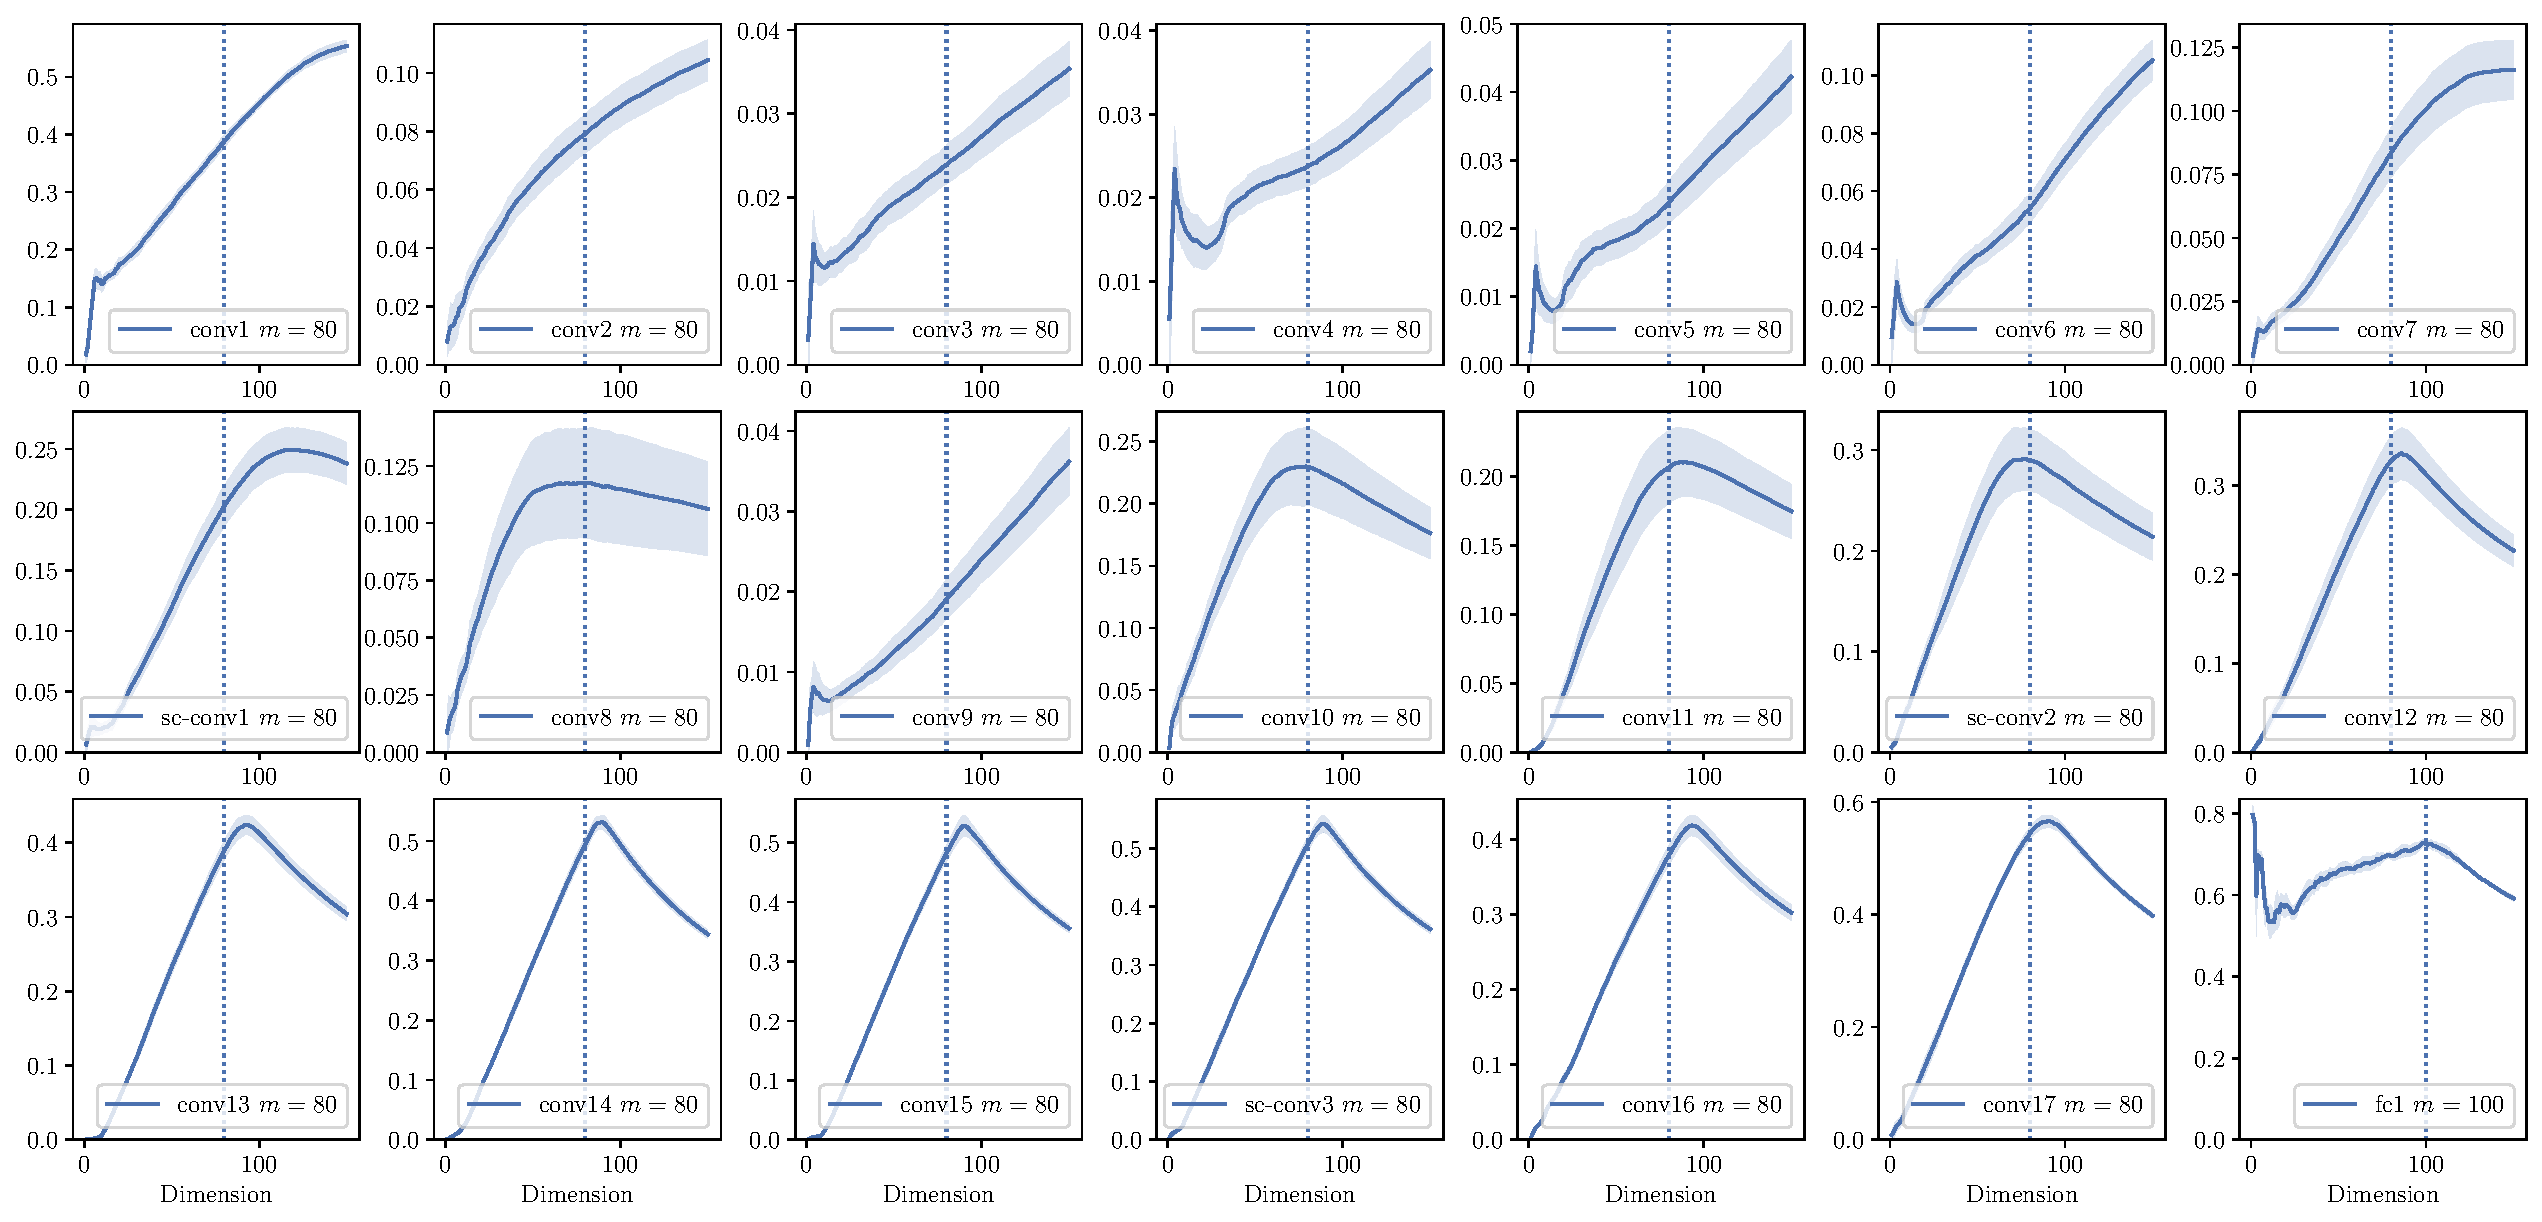
\includegraphics[width=\textwidth]{Appendix_Figures/Overlap_large_model/overlap_raw/ResNet/Resnet18W80_nobn_fixlr0.01_appendix_vertical_7col.pdf}
        \caption{ResNet18-W80 (CIFAR100)}
        \label{fig:app_adexp_cifar100_resnet80}
    \end{subfigure}
    \captionsetup{justification=centering}
    \caption{Top Eigenspace overlap for variants of ResNet18 on CIFAR100}
    \label{fig:app_adexp_resnet}
\end{figure}


\subsubsection{Failed cases for eigenspace overlap}
\label{sec:appendix-failed-exp}
As seen in \figureref{fig:app_adexp_vgg} and \figureref{fig:app_adexp_resnet}, there is a small portion of layers, usually closer to the input, whose eigenspace overlap does peak around the output dimensions. These layers can be clustered into the following two general cases.


\paragraph{Early Peak of Low Overlap}
For layers shown in \figureref{fig:app_adexp_failure_early}. The overlap of dominating eigenspaces are significantly lower than the other layers. Also there exists a small peak at very small dimensions.

% \begin{figure}[H]
%     \centering
%     \subfigure[\centering\small{fc2:F-$200^2$\\(MNIST)}]{
%     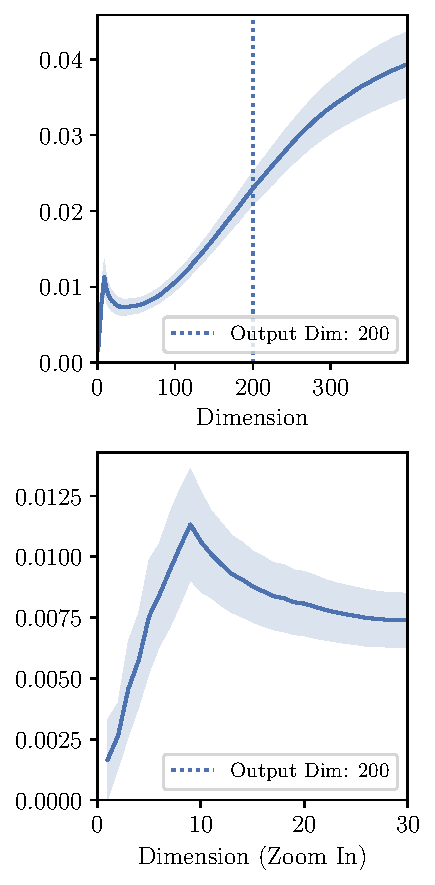
\includegraphics[width=0.23\textwidth]{Appendix_Figures/Overlap_large_model/FailCases/early/FC2_fixlr0.01_fc2_zoom_stacked.pdf}}
%     \subfigure[\centering\small{conv5:VGG11-W200\\(CIFAR10)}]{
%     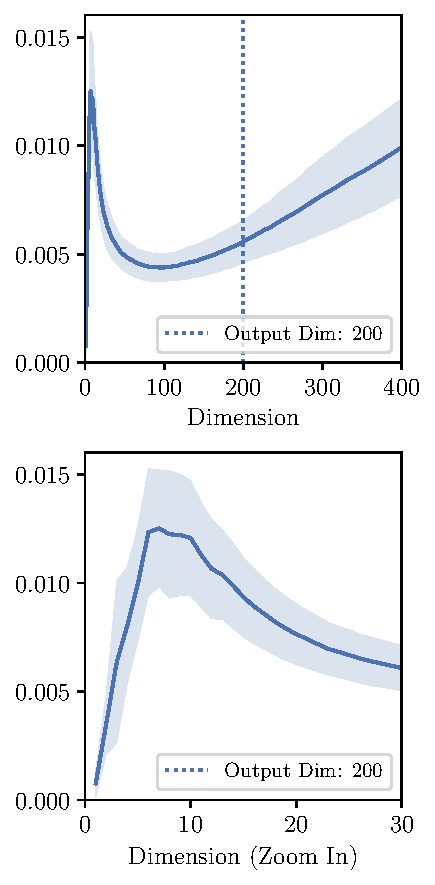
\includegraphics[width=0.23\textwidth]{Appendix_Figures/Overlap_large_model/FailCases/early/CIFAR10_VGG11W200_fxlr0.01_conv5_zoom_stacked.pdf}}
%     \subfigure[\centering\small{conv2:VGG11-W80\\(CIFAR100)}]{
%     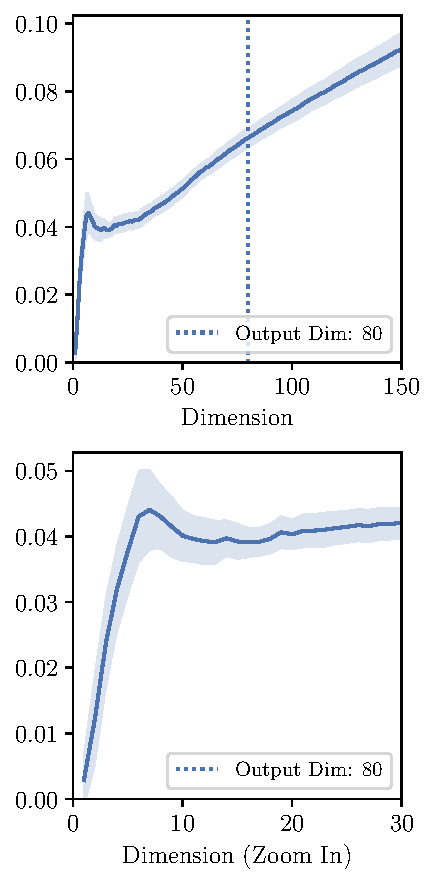
\includegraphics[width=0.23\textwidth]{Appendix_Figures/Overlap_large_model/FailCases/early/CIFAR100_VGG11W80New_nobn_fixlr0.01_conv2_zoom_stacked.pdf}}
%     \subfigure[\centering\small{conv5:RN18-W64\\(CIFAR100)}]{
%     \includegraphics[width=0.23\textwidth]{Appendix_Figures/Overlap_large_model/FailCases/early/CIFAR100_ResNet18W80_nobn_fixlr0.01_conv5_zoom_stacked.pdf}}
%     \caption{Top eigenspace overlap for layers with an early low peak. Figures in the second row are the zoomed in versions of the figures in the first row. (RN denotes ResNet in (\emph{d}))}
%     \label{fig:app_adexp_failure_early}
% \end{figure}

\begin{figure}[h]
    \centering
    \begin{subfigure}[b]{0.23\textwidth}
        \centering
        \captionsetup{justification=centering}
        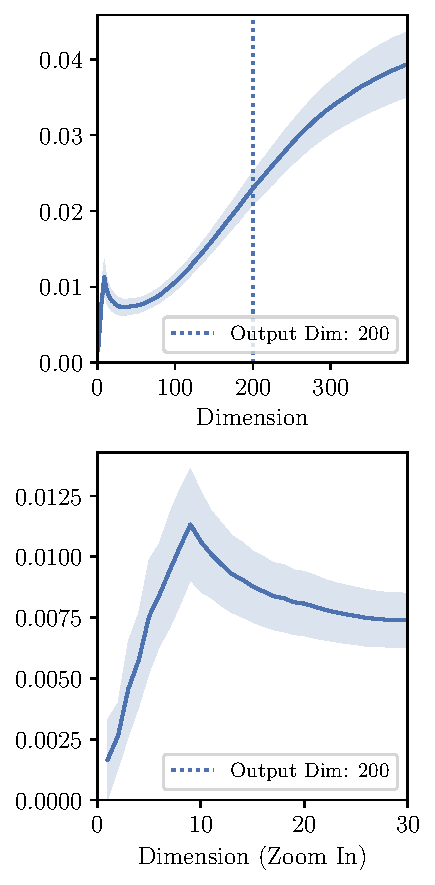
\includegraphics[width=\textwidth]{Appendix_Figures/Overlap_large_model/FailCases/early/FC2_fixlr0.01_fc2_zoom_stacked.pdf}
        \caption{fc2:F-$200^2$\\(MNIST)}
        \label{fig:app_adexp_overlap_early_mnistfc2}
    \end{subfigure}
    \begin{subfigure}[b]{0.23\textwidth}
        \centering
        \captionsetup{justification=centering}
        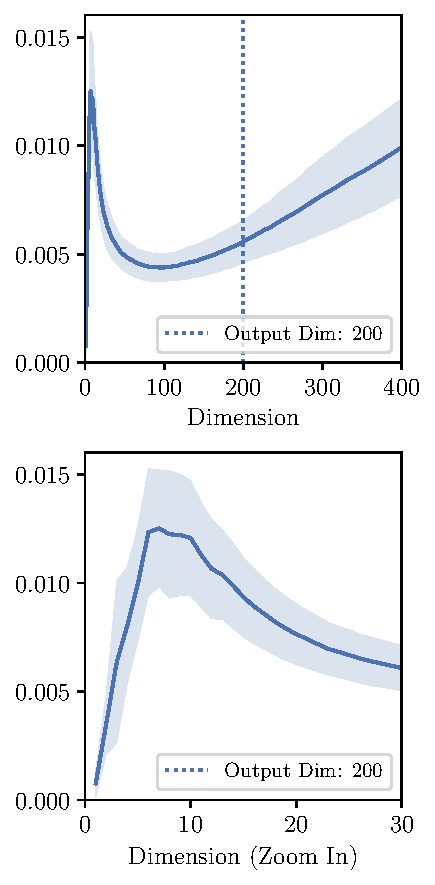
\includegraphics[width=\textwidth]{Appendix_Figures/Overlap_large_model/FailCases/early/CIFAR10_VGG11W200_fxlr0.01_conv5_zoom_stacked.pdf}
        \caption{conv5:VGG11-W200\\(CIFAR10)}
        \label{fig:app_adexp_overlap_early_vgg_cifar10}
    \end{subfigure}
    \begin{subfigure}[b]{0.23\textwidth}
        \centering
        \captionsetup{justification=centering}
        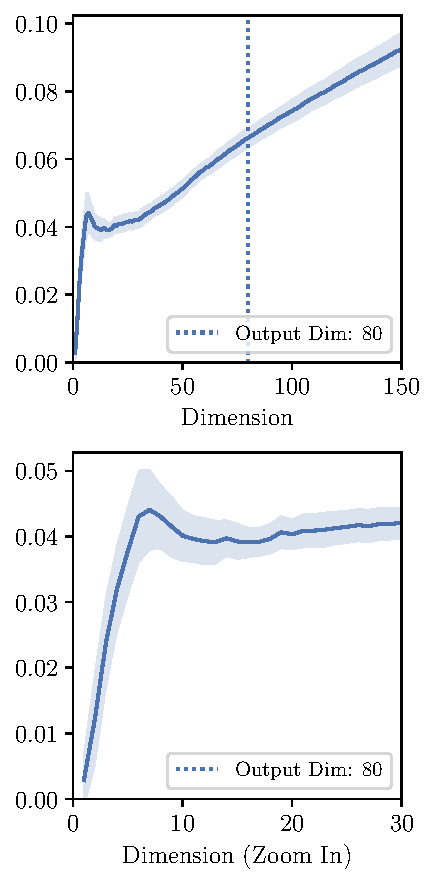
\includegraphics[width=\textwidth]{Appendix_Figures/Overlap_large_model/FailCases/early/CIFAR100_VGG11W80New_nobn_fixlr0.01_conv2_zoom_stacked.pdf}
        \caption{conv2:VGG11-W80\\(CIFAR100)}
        \label{fig:app_adexp_overlap_early_vgg_cifar100}
    \end{subfigure}
    \begin{subfigure}[b]{0.23\textwidth}
        \centering
        \captionsetup{justification=centering}
        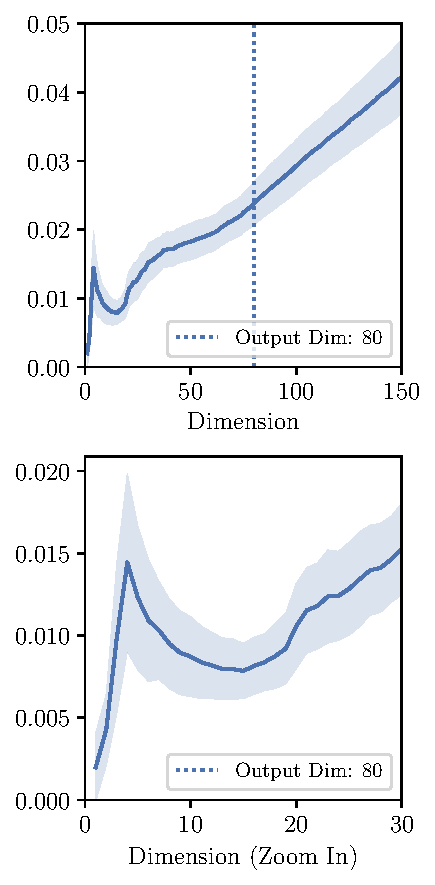
\includegraphics[width=\textwidth]{Appendix_Figures/Overlap_large_model/FailCases/early/CIFAR100_Resnet18W80_nobn_fixlr0.01_conv5_zoom_stacked.pdf}
        \caption{conv5:ResNet18-W64\\(CIFAR100)}
        \label{fig:app_adexp_overlap_early_resnet}
    \end{subfigure}
    \captionsetup{justification=centering}
    \caption{Top eigenspace overlap for layers with an early low peak.\\Figures in the second row are the zoomed in versions of the figures in the first row.}
    \label{fig:app_adexp_failure_early}
\end{figure}

\paragraph{Delayed Peak / Peak Doesn't Decline} 
For layers shown in \figureref{fig:app_adexp_failure_late}, the top eigenspaces has a nontrivial overlap, but the peak dimension is larger than predicted output dimension.

% \begin{figure}[H]
%     \centering
%     \subfigure[\centering\small{conv2:VGG11-W200\\(CIFAR10)}]{
%     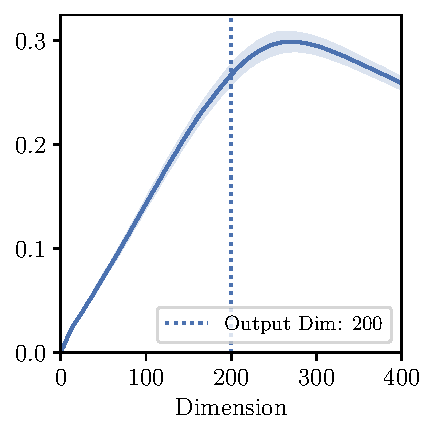
\includegraphics[width=0.23\textwidth]{Appendix_Figures/Overlap_large_model/FailCases/late/CIFAR10_VGG11W200_fxlr0.01_conv2.pdf}}
%     \subfigure[\centering\small{conv7:VGG11-W48\\(CIFAR100)}]{
%     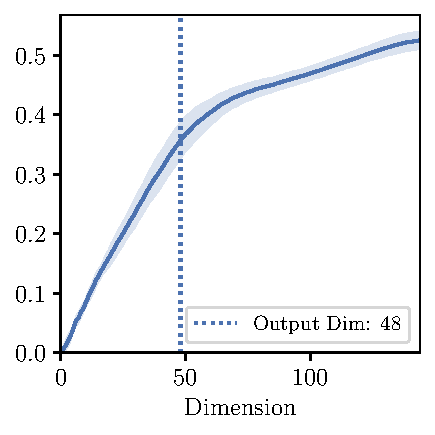
\includegraphics[width=0.23\textwidth]{Appendix_Figures/Overlap_large_model/FailCases/late/CIFAR100_VGG11W48New_nobn_fixlr0.01_conv7.pdf}}
%     \subfigure[\centering\small{conv7:RN18-W48\\(CIFAR100)}]{
%     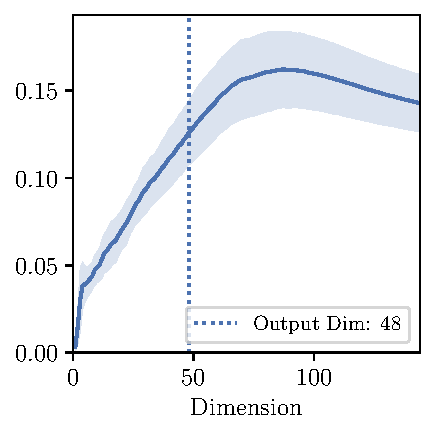
\includegraphics[width=0.23\textwidth]{Appendix_Figures/Overlap_large_model/FailCases/late/CIFAR100_Resnet18W48New_nobn_fixlr0.01_conv7.pdf}}
%     \subfigure[\centering\small{conv7:RN18-W64\\(CIFAR100)}]{
%     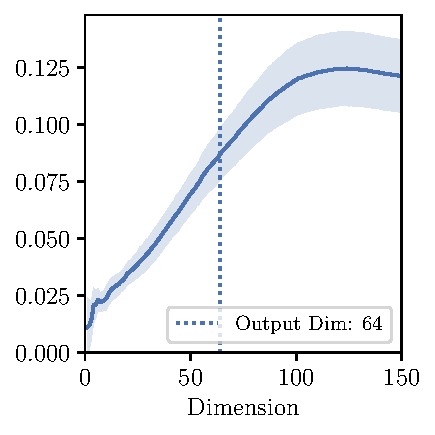
\includegraphics[width=0.23\textwidth]{Appendix_Figures/Overlap_large_model/FailCases/late/CIFAR100_Resnet18W64New_nobn_fixlr0.01_conv7.pdf}}
%     \caption{Top eigenspace overlap for layers with a delayed peak (RN denotes ResNet).}
%     \label{fig:app_adexp_failure_late}
% \end{figure}

\begin{figure}[h]
    \centering
    \begin{subfigure}[b]{0.23\textwidth}
        \centering
        \captionsetup{justification=centering}
        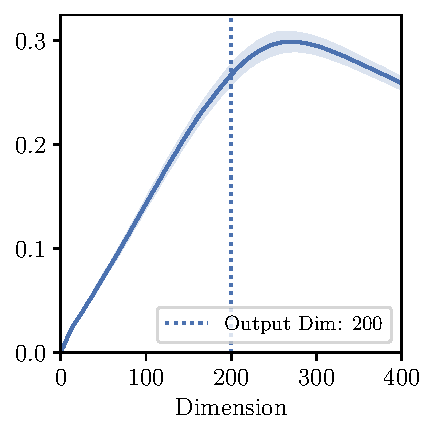
\includegraphics[width=\textwidth]{Appendix_Figures/Overlap_large_model/FailCases/late/CIFAR10_VGG11W200_fxlr0.01_conv2.pdf}
        \caption{conv2:VGG11-W200\\(CIFAR10)}
        \label{fig:app_adexp_overlap_late_vgg_cifar10}
    \end{subfigure}
    \begin{subfigure}[b]{0.23\textwidth}
        \centering
        \captionsetup{justification=centering}
        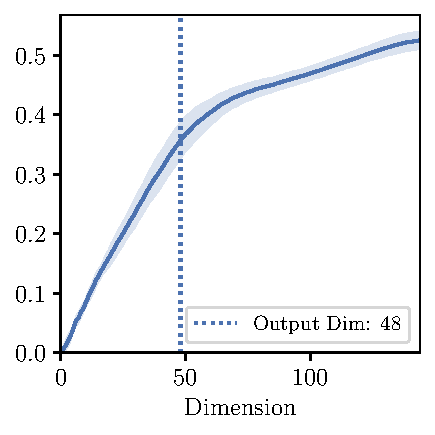
\includegraphics[width=\textwidth]{Appendix_Figures/Overlap_large_model/FailCases/late/CIFAR100_VGG11W48New_nobn_fixlr0.01_conv7.pdf}
        \caption{conv7:VGG11-W48\\(CIFAR100)}
        \label{fig:app_adexp_overlap_late_vgg_cifar100}
    \end{subfigure}
    \begin{subfigure}[b]{0.23\textwidth}
        \centering
        \captionsetup{justification=centering}
        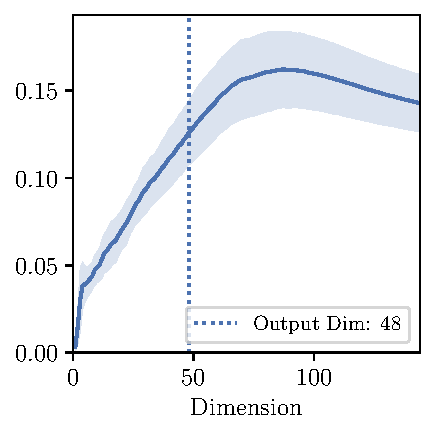
\includegraphics[width=\textwidth]{Appendix_Figures/Overlap_large_model/FailCases/late/CIFAR100_Resnet18W48New_nobn_fixlr0.01_conv7.pdf}
        \caption{conv7:VGG11-W48\\(CIFAR100)}
        \label{fig:app_adexp_overlap_late_resnet48}
    \end{subfigure}
    \begin{subfigure}[b]{0.23\textwidth}
        \centering
        \captionsetup{justification=centering}
        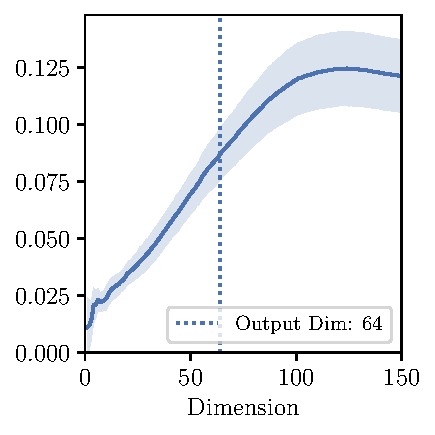
\includegraphics[width=\textwidth]{Appendix_Figures/Overlap_large_model/FailCases/late/CIFAR100_Resnet18W64New_nobn_fixlr0.01_conv7.pdf}
        \caption{conv7:ResNet18-W64\\(CIFAR100)}
        \label{fig:app_adexp_overlap_late_resnet}
    \end{subfigure}
    \captionsetup{justification=centering}
    \caption{Top eigenspace overlap for layers with a delayed peak.}
    \label{fig:app_adexp_failure_late}
\end{figure}

However, the existence of such failure cases \emph{does not} undermine the theory of Kronecker factorization approximation. In fact, both appear because the top hessian eigenspace is not completely spanned by $\E[\vx]$,  and can be predicted by computing the auto correlation matrices and the output Hessians. The details will also be elaborated in \sectionref{sec:appendix_model_overlap} with the help of correspondence matrices.

% \paragraph{Overlap may exhibits a early peak for some layers:} For the eigenspace overlap plot of F-$200^2$ (\figureref{fig:app_overlap_fail}), we see that the overlap for fc2 is significantly lower than the other layers, and there exists a small peak near dimension $k=10$. This is because the top hessian eigenspace is not completely spanned by $\E[\vx]$. This phenomenon will also be elaborated in \sectionref{sec:appendix_model_overlap} with the help of correspondence matrices.
% \begin{figure}[h]
%     \centering
%     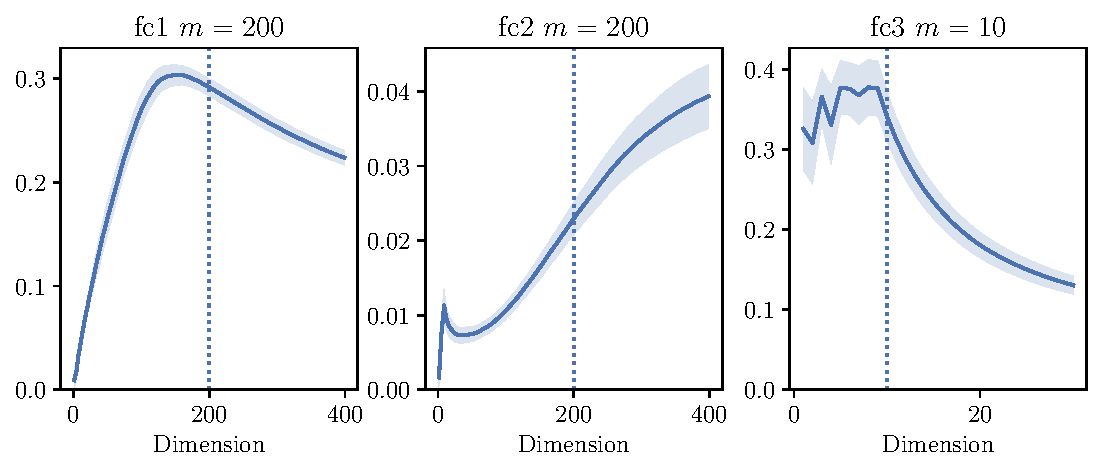
\includegraphics[width=0.6\textwidth]{Appendix_Figures/Overlap_different_models/DimOverlap_MNIST_FC2_fixlr0.01_appendix_full.pdf}
%     \caption{Eigenspace overlap of different models of F-$200^2$.}
%     \label{fig:app_overlap_fail}

% \end{figure}
